\chapter{Anexos}\label{anexos}

\section{Diccionario de datos de la base original}
\label{sec:diccionario-datos}

Este anexo documenta la estructura y el contenido del archivo fuente
\texttt{Siniestros unificados para nuevas variables julio 2025 v9 con distancias},
provisto por el equipo de datos del Ministerio Público Fiscal. Se reproducen los
nombres de campo tal como figuran en la planilla original, aun cuando su grafía no
sea homogénea, para preservar la trazabilidad con la fuente.

\subsection{Estructura de la planilla}
\label{ssec:estructura-planilla}

La base se organiza en tres niveles de análisis: el hecho siniestro, las personas
involucradas y la georreferenciación. Todas las hojas se vinculan por el número de
expediente (SAC), que opera como identificador único del siniestro.

\begin{table}[H]
\centering
\caption{Hojas que componen la planilla de cálculo original}
\label{tab:hojas-planilla}
\begin{tabular}{@{}>{\raggedright\arraybackslash}p{0.26\textwidth}
                  >{\raggedright\arraybackslash}p{0.52\textwidth}
                  >{\raggedleft\arraybackslash}p{0.12\textwidth}@{}}
\toprule
\textbf{Hoja} & \textbf{Contenido} & \textbf{Registros} \\
\midrule
\texttt{HECHO} & Siniestros con todas las variables del nivel hecho & 4906 \\
\texttt{Hecho solo georreferencia} & Subconjunto de siniestros efectivamente geocodificados & 4321 \\
\texttt{Códigos} & Catálogo de referencias de codificación de las hojas de hecho & --- \\
\texttt{Víctimas} & Datos simples de víctimas (sexo al nacer y edad simple) & 5673 \\
\texttt{Victagregada} & Víctimas agregadas por sexo al nacer y grupo etario & 4820 \\
\texttt{Denunciados} & Datos simples de denunciados (sexo al nacer y edad simple) & 5011 \\
\texttt{Denagregada} & Denunciados agregados por sexo al nacer y grupo etario & 4257 \\
\texttt{Personas} & Unión de víctimas y denunciados con una columna de rol & 10\,684 \\
\texttt{Georreferenciación} & Siniestros revisados en el proceso de geocodificación manual & 4884 \\
\bottomrule
\end{tabular}

\vspace{0.5em}
{\footnotesize \textit{Nota}. Elaboración propia sobre la planilla provista por el
Ministerio Público Fiscal. Cuando un mismo número de SAC correspondía a domicilios
distintos ---y por lo tanto a siniestros distintos--- se le añadió el sufijo
\texttt{.1} para desambiguarlo.}
\end{table}

\subsection{Variables de la base de datos}
\label{ssec:variables-hecho}

\begin{longtable}{@{}>{\raggedright\arraybackslash}p{0.23\textwidth}
                    >{\raggedright\arraybackslash}p{0.44\textwidth}
                    >{\raggedright\arraybackslash}p{0.26\textwidth}@{}}
\caption{Diccionario de datos}
\label{tab:diccionario-hecho} \\
\toprule
\textbf{Variable} & \textbf{Descripción} & \textbf{Valores o codificación} \\
\midrule
\endfirsthead

\multicolumn{3}{@{}l}{\footnotesize\textit{Tabla \ref{tab:diccionario-hecho} (continuación)}} \\
\toprule
\textbf{Variable} & \textbf{Descripción} & \textbf{Valores o codificación} \\
\midrule
\endhead

\midrule
\multicolumn{3}{r@{}}{\footnotesize\textit{Continúa en la página siguiente}} \\
\endfoot

\bottomrule
\endlastfoot

\multicolumn{3}{@{}l}{\textit{Identificación y variables temporales}} \\
\addlinespace
\texttt{Nro.\ de SAC} & Número de expediente; identificador único del siniestro & Alfanumérico \\
\texttt{Fecha de ingreso} & Fecha de ingreso del expediente, aproximada a la del siniestro & Fecha \\
\texttt{Hora del hecho} & Hora real del siniestro consignada en el expediente & Formato 24 h \\
\texttt{franja\_horaria} & Bloque horario de seis horas en que ocurre el siniestro & 1 = madrugada (0--6 h); 2 = mañana (6--12 h); 3 = tarde (12--18 h); 4 = noche (18--24 h) \\
\texttt{dia\_semana\_cat} & Día de la semana & 1 = lunes \ldots\ 7 = domingo \\
\texttt{es\_fin\_de\_semana} & Indica si el siniestro ocurre en fin de semana & 1 = sí; 2 = no \\
\texttt{es\_hora\_punta} & Indica si el siniestro ocurre en hora pico & 1 = sí (7:30--9:30, 12:00--14:00 y 17:30--19:30 h); 2 = no \\
\texttt{tipomesESCOLAR} & Régimen del mes según el calendario escolar y laboral & 1 = laboral/escolar (marzo a noviembre); 2 = no laboral (diciembre a febrero) \\
\texttt{estacionCLIMA} & Estación del año & 1 = otoño; 2 = invierno; 3 = primavera; 4 = verano \\
\addlinespace

\multicolumn{3}{@{}l}{\textit{Consecuencias del siniestro}} \\
\addlinespace
\texttt{Lesiones} & Tipo de lesiones según la carátula del expediente & Texto libre \\
\texttt{Lesionescod} & Codificación del tipo de lesiones & 1 = leves; 2 = graves; 3 = homicidio; 4 = otras \\
\addlinespace

\multicolumn{3}{@{}l}{\textit{Vehículos involucrados}} \\
\addlinespace
\texttt{Vehículo} & Vehículo 1 involucrado en el hecho & Texto libre \\
\texttt{VEHICULO1COD} & Codificación del vehículo 1 & Entero \\
\texttt{Vehiculo2} & Vehículo 2 o combinación de vehículos; los múltiples se separan con guion medio & Texto libre \\
\texttt{VEHICULO2COD} & Codificación del vehículo 2; se toma el más pesado del conjunto & Entero \\
\texttt{Transporte publico1} & Indica si el vehículo 1 es transporte público de pasajeros (colectivo, trolebús) & 1 = sí; 2 = no \\
\texttt{Transporte publico2} & Indica si el vehículo 2 es transporte público de pasajeros & 1 = sí; 2 = no \\
\texttt{Inmovil1} & Indica si el vehículo 1 es un objeto fijo (árbol, pared, reja, poste) & 1 = sí; 2 = no \\
\texttt{Inmovil2} & Indica si el vehículo 2 es un objeto fijo & 1 = sí; 2 = no \\
\texttt{Motorizado1} & Indica si el vehículo 1 es motorizado & 1 = sí; 2 = no \\
\texttt{Motorizado2} & Indica si el vehículo 2 es motorizado & 1 = sí; 2 = no \\
\texttt{Tamaño1} & Tamaño del vehículo 1 según su peso aproximado & Texto libre \\
\texttt{tam1cod} & Codificación del tamaño del vehículo 1 & 1 = persona; 2 = ligero; 3 = mediano; 4 = medio pesado; 5 = pesado \\
\texttt{Tamaño2} & Tamaño del vehículo 2 según su peso aproximado & Texto libre \\
\texttt{tam2cod} & Codificación del tamaño del vehículo 2 & 1 = persona; 2 = ligero; 3 = mediano; 4 = medio pesado; 5 = pesado \\
\texttt{TOTAL\_VEHICULOS} & Cantidad total de vehículos involucrados & Entero \\
\texttt{Complejidad} & Tipo de colisión según los actores involucrados & Texto libre \\
\texttt{Complejcod} & Codificación del tipo de colisión & 1 = casual o sin dato; 2 = dupla; 3 = múltiple \\
\texttt{involbici} & Indica si intervino al menos una bicicleta & 1 = sí; 2 = no \\
\texttt{involPeaton} & Indica si intervino al menos un peatón & 1 = sí; 2 = no \\
\addlinespace

\multicolumn{3}{@{}l}{\textit{Personas involucradas}} \\
\addlinespace
\texttt{V\_Fem} & Cantidad de víctimas de sexo femenino & Entero \\
\texttt{V\_Masc} & Cantidad de víctimas de sexo masculino & Entero \\
\texttt{V\_ninos} & Cantidad de víctimas del grupo etario niños & Entero \\
\texttt{V\_joven} & Cantidad de víctimas del grupo etario jóvenes & Entero \\
\texttt{V\_adulto} & Cantidad de víctimas del grupo etario adultos & Entero \\
\texttt{V\_adumayor} & Cantidad de víctimas del grupo etario adultos mayores & Entero \\
\texttt{D\_Fem} & Cantidad de denunciados de sexo femenino & Entero \\
\texttt{D\_Masc} & Cantidad de denunciados de sexo masculino & Entero \\
\texttt{D\_ninos} & Cantidad de denunciados del grupo etario niños & Entero \\
\texttt{D\_joven} & Cantidad de denunciados del grupo etario jóvenes & Entero \\
\texttt{D\_adulto} & Cantidad de denunciados del grupo etario adultos & Entero \\
\texttt{D\_adumayor} & Cantidad de denunciados del grupo etario adultos mayores & Entero \\
\texttt{victimas} & Cantidad total de víctimas del siniestro & Entero \\
\texttt{denunciados} & Cantidad total de denunciados del siniestro & Entero \\
\texttt{TotalPersonas} & Cantidad total de personas involucradas & Entero \\
\addlinespace

\multicolumn{3}{@{}l}{\textit{Localización y entorno vial}} \\
\addlinespace
\texttt{Latitud} & Latitud del punto de ocurrencia & Grados decimales \\
\texttt{Longitud} & Longitud del punto de ocurrencia & Grados decimales \\
\texttt{tipoVÍA} & Clasificación de la red vial según la ordenanza municipal 8060 & Texto libre \\
\texttt{TIPOVIA2} & Jerarquía de la vía, con bandas de 20 metros & Vía arterial-sectorial; vías de barrio \\
\texttt{Num Semáforo} & Identificador del semáforo más cercano & Alfanumérico \\
\texttt{Distancia Semáforo METROS} & Distancia radial al semáforo más cercano & Metros \\
\texttt{ConSemaforo} & Indica si hay un semáforo a 100 metros o menos & 1 = sí; 2 = no \\
\texttt{IDVERTICE} & Identificador del vértice (esquina) más cercano & Alfanumérico \\
\texttt{DIST VERTICE METROS} & Distancia radial a la esquina más cercana & Metros \\
\texttt{Enesquina} & Indica si el siniestro ocurrió a 15 metros o menos de un vértice & 1 = sí; 2 = no \\
\texttt{IDLUMINARIA} & Identificador de la luminaria más cercana & Alfanumérico \\
\texttt{DIST LUMINARIA METROS} & Distancia radial a la luminaria más cercana & Metros \\
\addlinespace

\multicolumn{3}{@{}l}{\textit{Condiciones solares y de luminosidad}} \\
\addlinespace
\texttt{amanece} & Hora de inicio del crepúsculo matutino & Formato 24 h \\
\texttt{salidasol} & Hora de salida del sol & Formato 24 h \\
\texttt{acimut1} & Acimut solar en la salida del sol, medido en sentido horario desde el norte geográfico & Grados (0--360) \\
\texttt{mediodía} & Hora en que el sol alcanza el cenit & Formato 24 h \\
\texttt{anochece} & Hora de inicio del crepúsculo vespertino & Formato 24 h \\
\texttt{acimut2} & Acimut solar en la puesta del sol, medido en sentido horario desde el norte geográfico & Grados (0--360) \\
\texttt{puesta} & Hora de puesta del sol & Formato 24 h \\
\texttt{horasxdia} & Duración total de la luz solar del día & Horas \\
\texttt{dianoche} & Indica si el siniestro ocurrió dentro o fuera del horario solar & Dentro del horario solar; fuera del horario solar \\
\texttt{LUMI\_NOCHE} & Disponibilidad de luminaria a 15 metros o menos en siniestros nocturnos & No había luminaria; es día, no usa luminaria; había luminaria \\
\end{longtable}

{\footnotesize \textit{Nota}. Elaboración propia sobre el documento de descripción de
datos provisto por el Ministerio Público Fiscal. Los nombres de campo se reproducen
con la grafía de la planilla original.}

\subsection{Notas metodológicas de la fuente}
\label{ssec:notas-fuente}

\paragraph{Georreferenciación.} La geocodificación se realizó de forma manual, caso por
caso, ubicando cada siniestro sobre cartografía en línea y registrando las coordenadas
de latitud y longitud. De los 4906 expedientes identificados como siniestros, 585 no
pudieron ubicarse con precisión ---mayoritariamente hechos sobre rutas referenciadas por
altura kilométrica o con descripciones ambiguas de la ubicación--- y 5 correspondían a
otra localidad. Quedaron así 4321 siniestros georreferenciados dentro del ejido de la
ciudad de Córdoba.

\paragraph{Clasificación de vehículos.} Se leyeron individualmente algo más de 9000
registros de expediente para identificar y clasificar los vehículos intervinientes
(automóvil, colectivo, motocicleta, utilitario, camión, entre otros). En ese proceso se
detectaron siniestros de tipo casual, con un único vehículo involucrado contra un objeto
inmóvil.

\paragraph{Grupos etarios.} La segmentación por edad sigue las recomendaciones de la
Organización Mundial de la Salud: niños (0 a 14 años), jóvenes (15 a 26 años), adultos
(27 a 59 años) y adultos mayores (60 años o más).

\paragraph{Variables solares.} Los horarios de salida y puesta del sol, crepúsculos,
acimut y duración del día se obtuvieron del \textit{Astronomical Applications Department}
del Observatorio Naval de los Estados Unidos, contrastados con los datos del Servicio de
Hidrografía Naval argentino. Se utilizó esa fuente por permitir la extracción tabular de
un año completo en una sola consulta, parametrizada para las coordenadas de la ciudad de
Córdoba.\footnote{\url{https://aa.usno.navy.mil/calculated/mrst}}

\paragraph{Revisión de variables.} En una instancia posterior de revisión se depuraron
las columnas de inmovilizados y las codificaciones redundantes; se unificó la
información de transporte público en una única variable de intervención, independiente
de la complejidad del hecho; y se redefinió la variable de complejidad como tipo de
colisión, con las categorías dupla (dos vehículos motorizados), múltiple (tres o más),
peatón contra vehículo motorizado, bicicleta contra vehículo motorizado, objeto contra
vehículo motorizado y otros. En la misma instancia se incorporaron las variables
\texttt{involbici} e \texttt{involPeaton}.

\section{Visualizaciones exploratorias complementarias}
\label{sec:visualizaciones-exploratorias}

Este anexo reúne el conjunto completo de visualizaciones generadas durante la etapa de
exploración de datos descripta en la \cref{exploraciuxf3n-de-datos}, sobre la base
consolidada de 4320 siniestros viales georreferenciados (julio de 2022 a junio de 2024).
Se incluyen aquí para no sobrecargar el cuerpo principal del informe, dado que solo una
selección de estas figuras se referencia directamente en el análisis.

\begin{figure}[htbp]
\centering
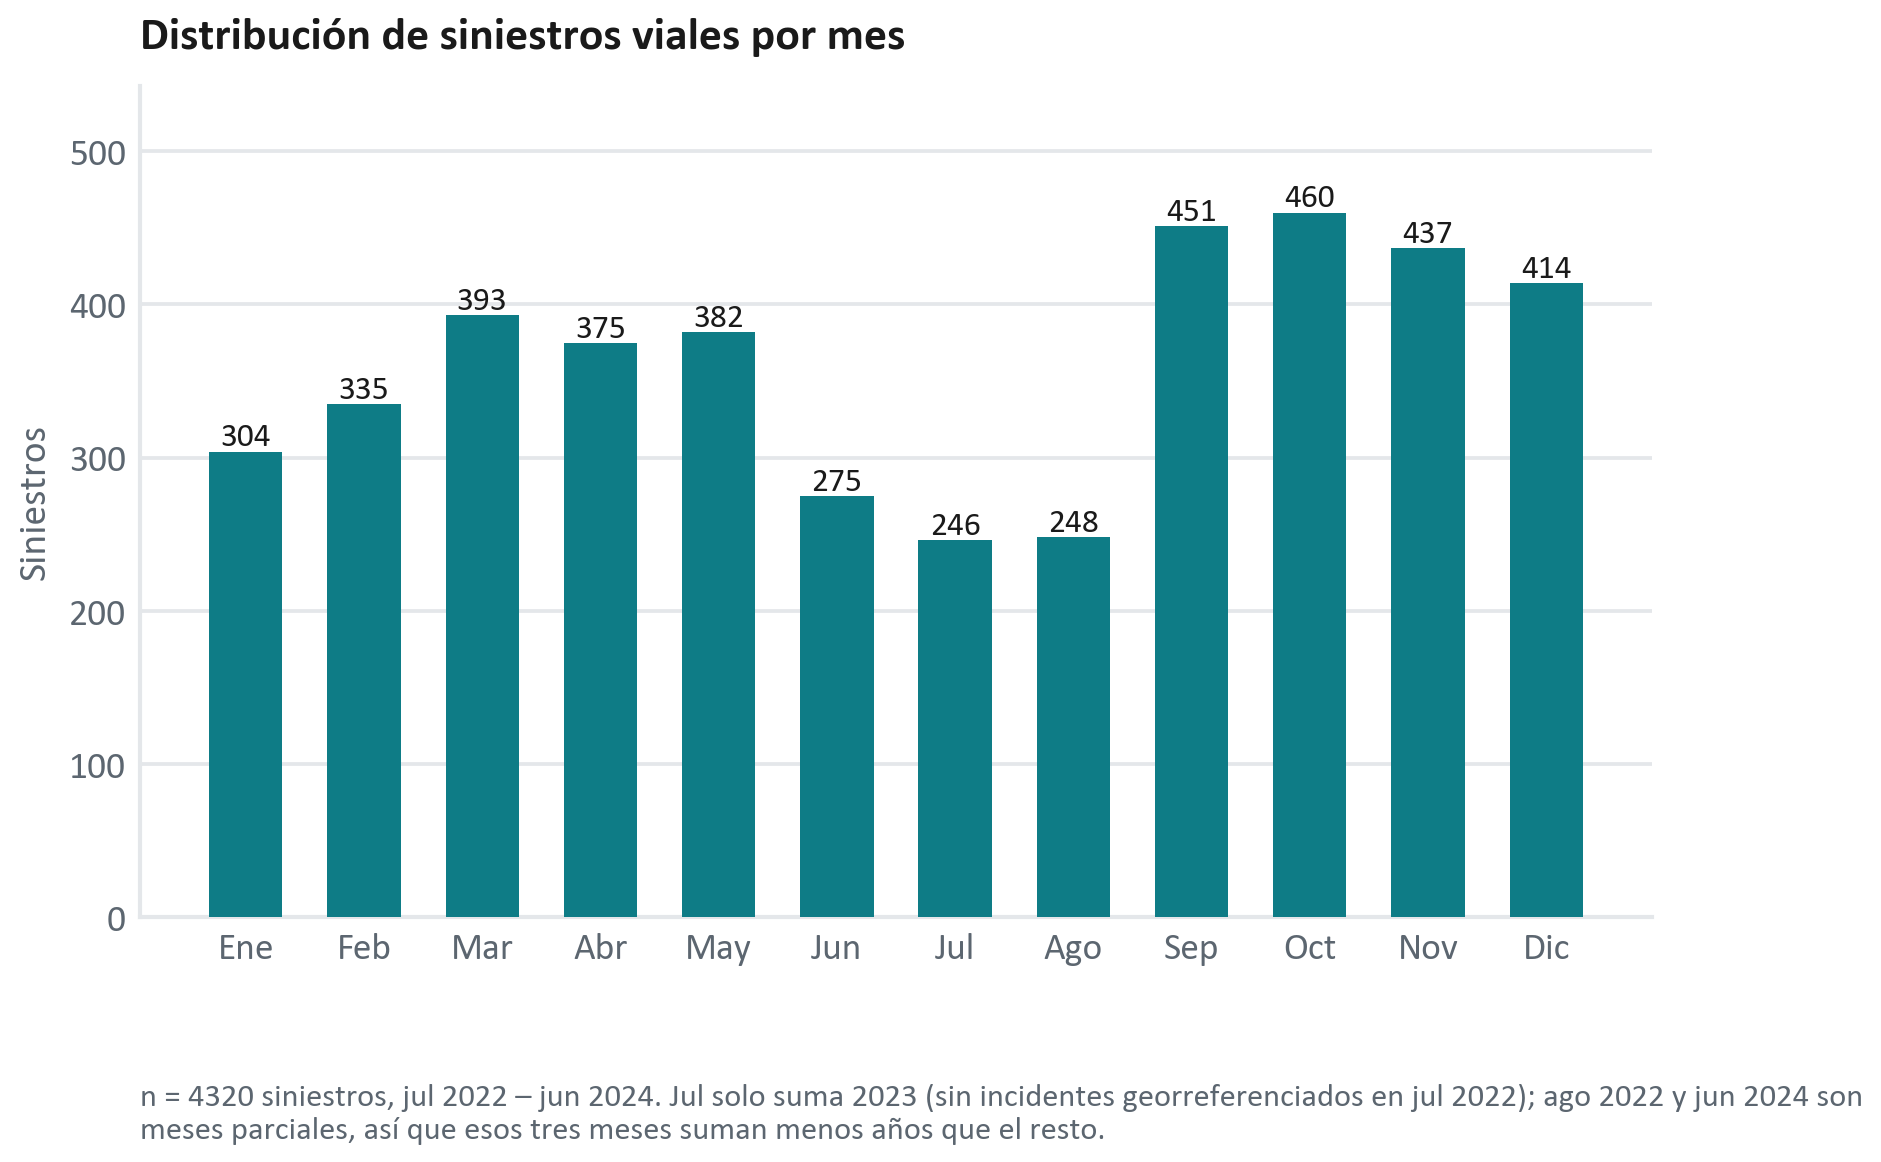
\includegraphics[width=0.85\linewidth]{imagenes/anexo_a2_distribucion_mes.png}
\caption{Distribución de siniestros viales por mes}
\label{fig:anexo-distribucion-mes}
\notaflot{Frecuencia mensual de siniestros georreferenciados (n = 4320), julio 2022 --
junio 2024. El máximo se registra en octubre (460) y el mínimo en julio (246); julio
computa únicamente 2023, y agosto de 2022 y junio de 2024 son meses parciales, por lo
que esos tres meses acumulan menos años que el resto. \fuentepropia{}.}
\end{figure}

\begin{figure}[htbp]
\centering
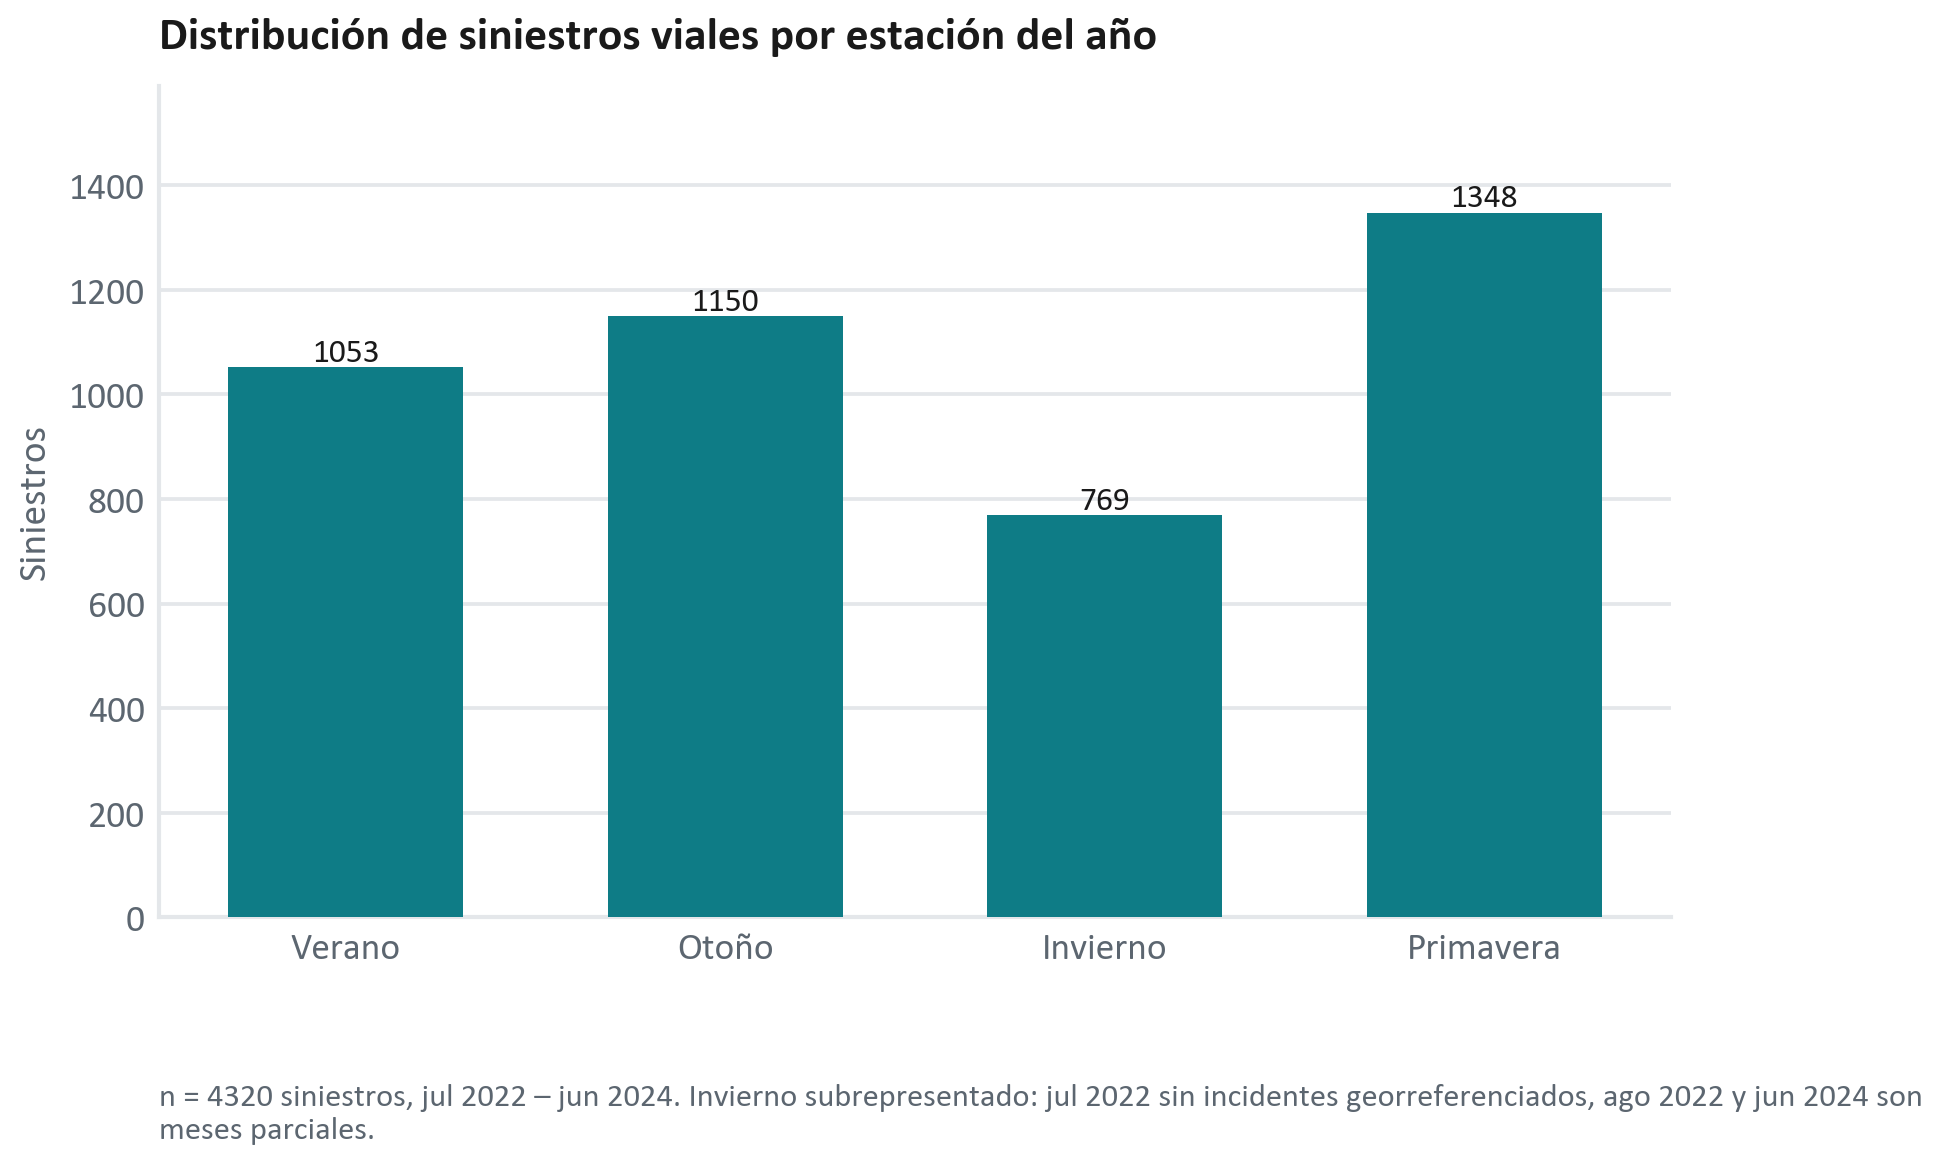
\includegraphics[width=0.8\linewidth]{imagenes/anexo_a2_distribucion_estacion.png}
\caption{Distribución de siniestros viales por estación del año}
\label{fig:anexo-distribucion-estacion}
\notaflot{Agregación estacional de los mismos 4320 siniestros. La primavera concentra
la mayor frecuencia (1348) y el invierno la menor (769), aunque esta última estación
está subrepresentada porque julio de 2022 no registra incidentes georreferenciados y
agosto de 2022 y junio de 2024 son meses parciales. \fuentepropia{}.}
\end{figure}

\begin{figure}[htbp]
\centering
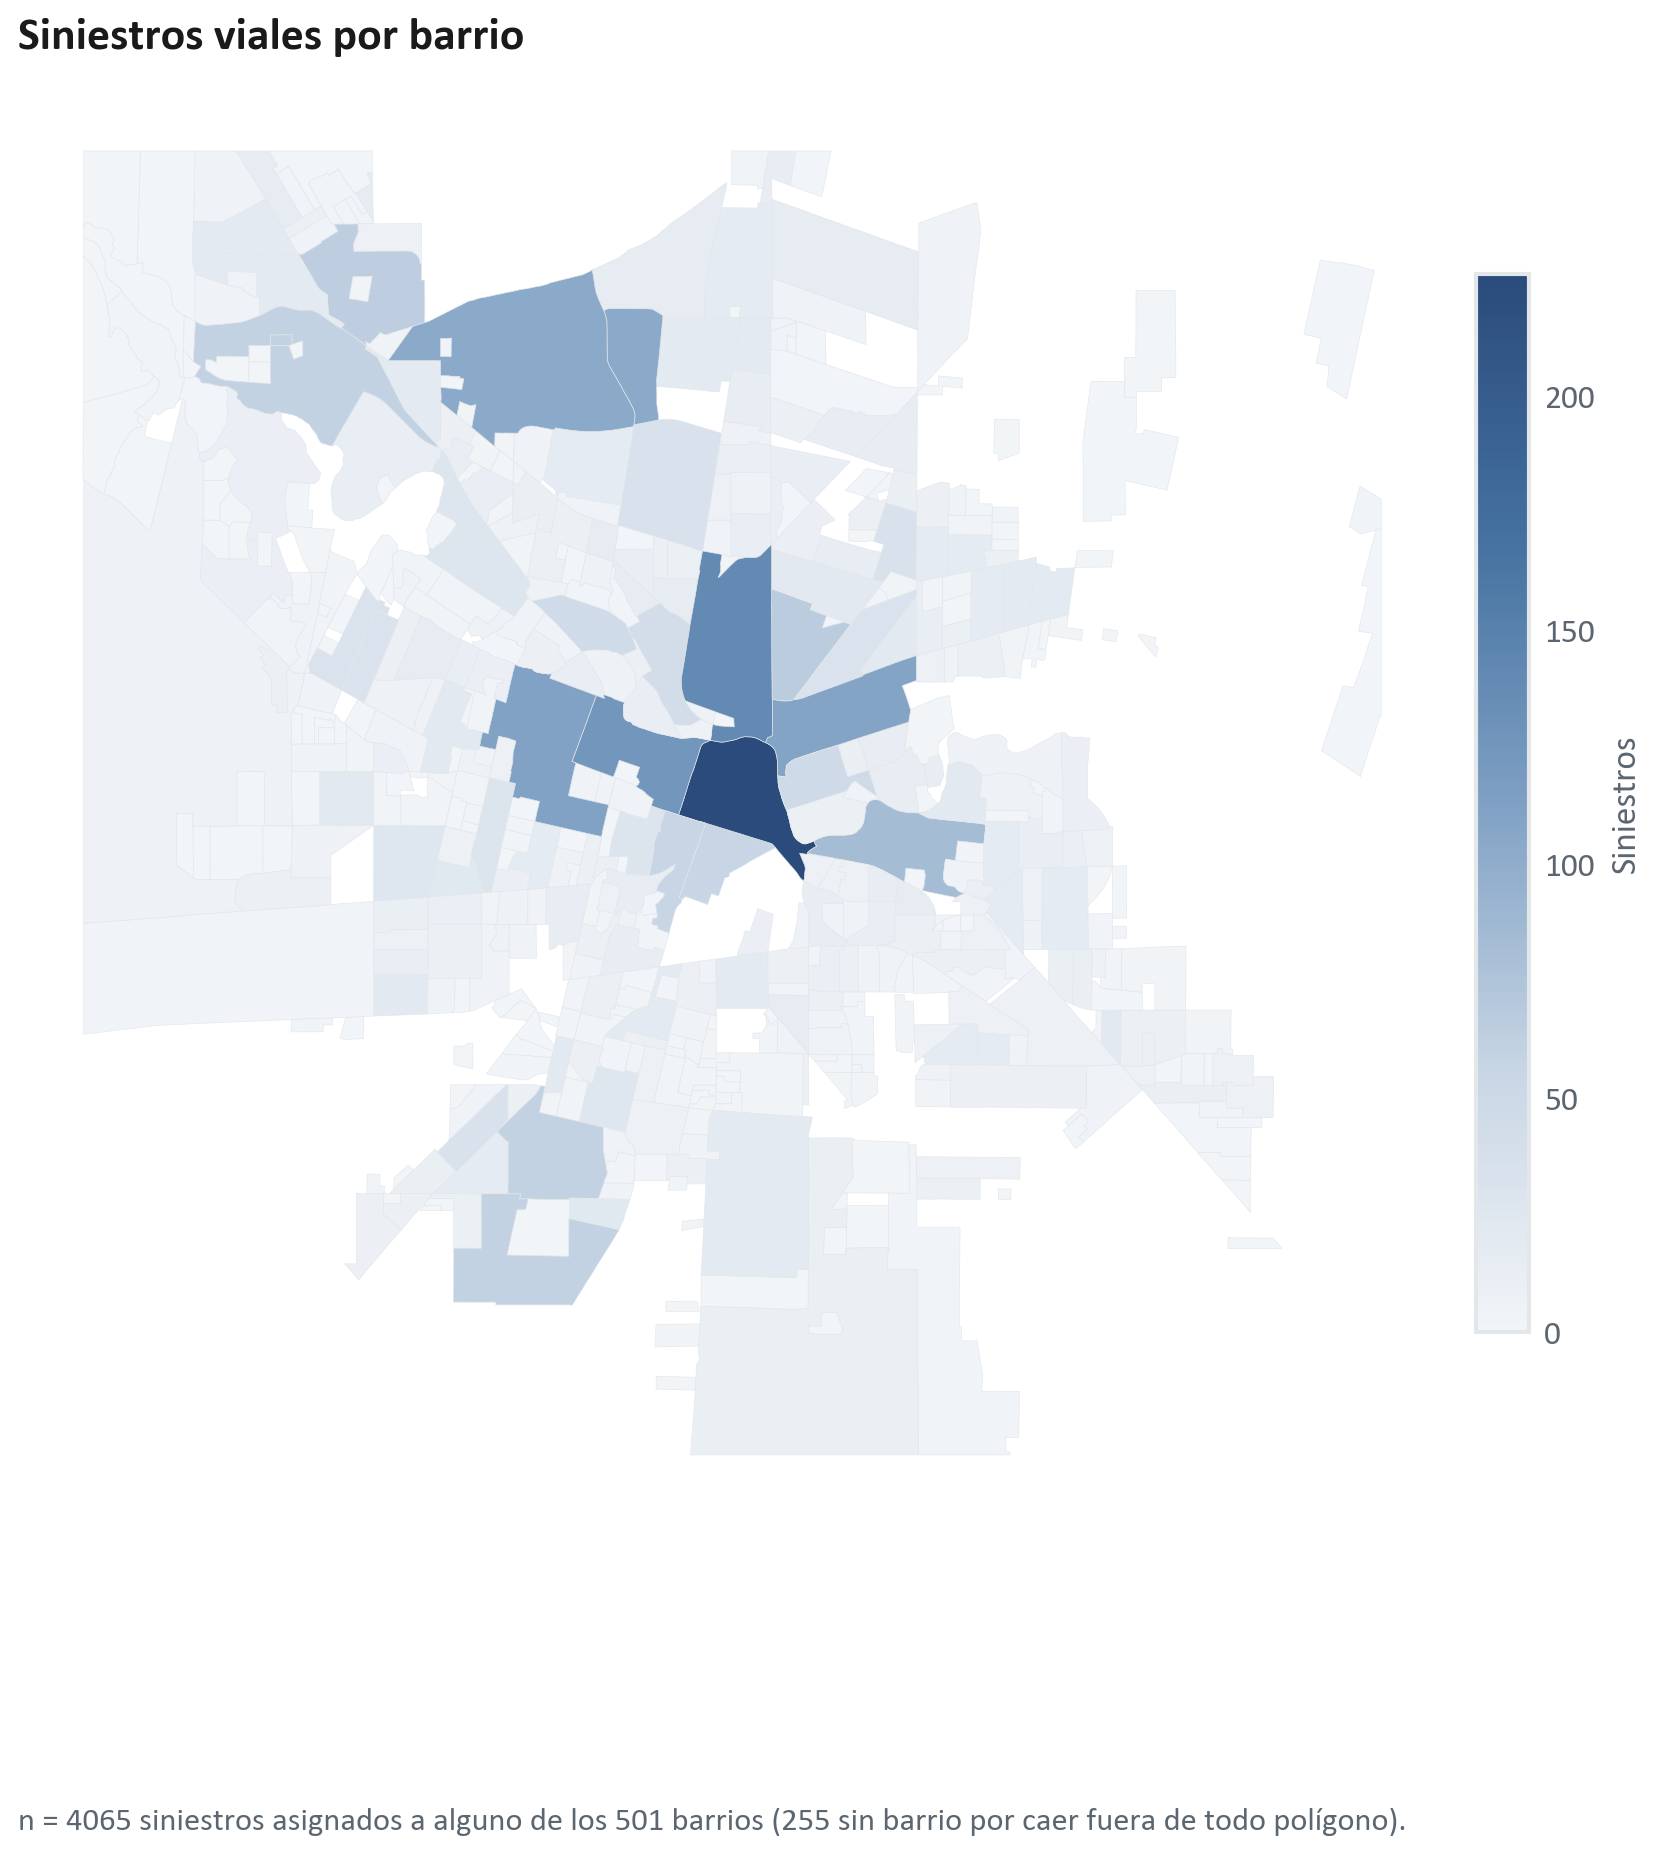
\includegraphics[width=0.62\linewidth]{imagenes/anexo_a2_mapa_calor_barrio.png}
\caption{Siniestros viales por barrio de la ciudad de Córdoba}
\label{fig:anexo-mapa-calor-barrio}
\notaflot{Cantidad de siniestros agregados por barrio (n = 4065 asignados a alguno de
los 501 polígonos vigentes; 255 casos cayeron fuera de todo polígono y quedaron sin
barrio asignado). El área central y sus barrios inmediatos concentran los valores más
altos, con un máximo superior a 200 siniestros en el polígono central. \fuentepropia{}.}
\end{figure}

\begin{figure}[htbp]
\centering
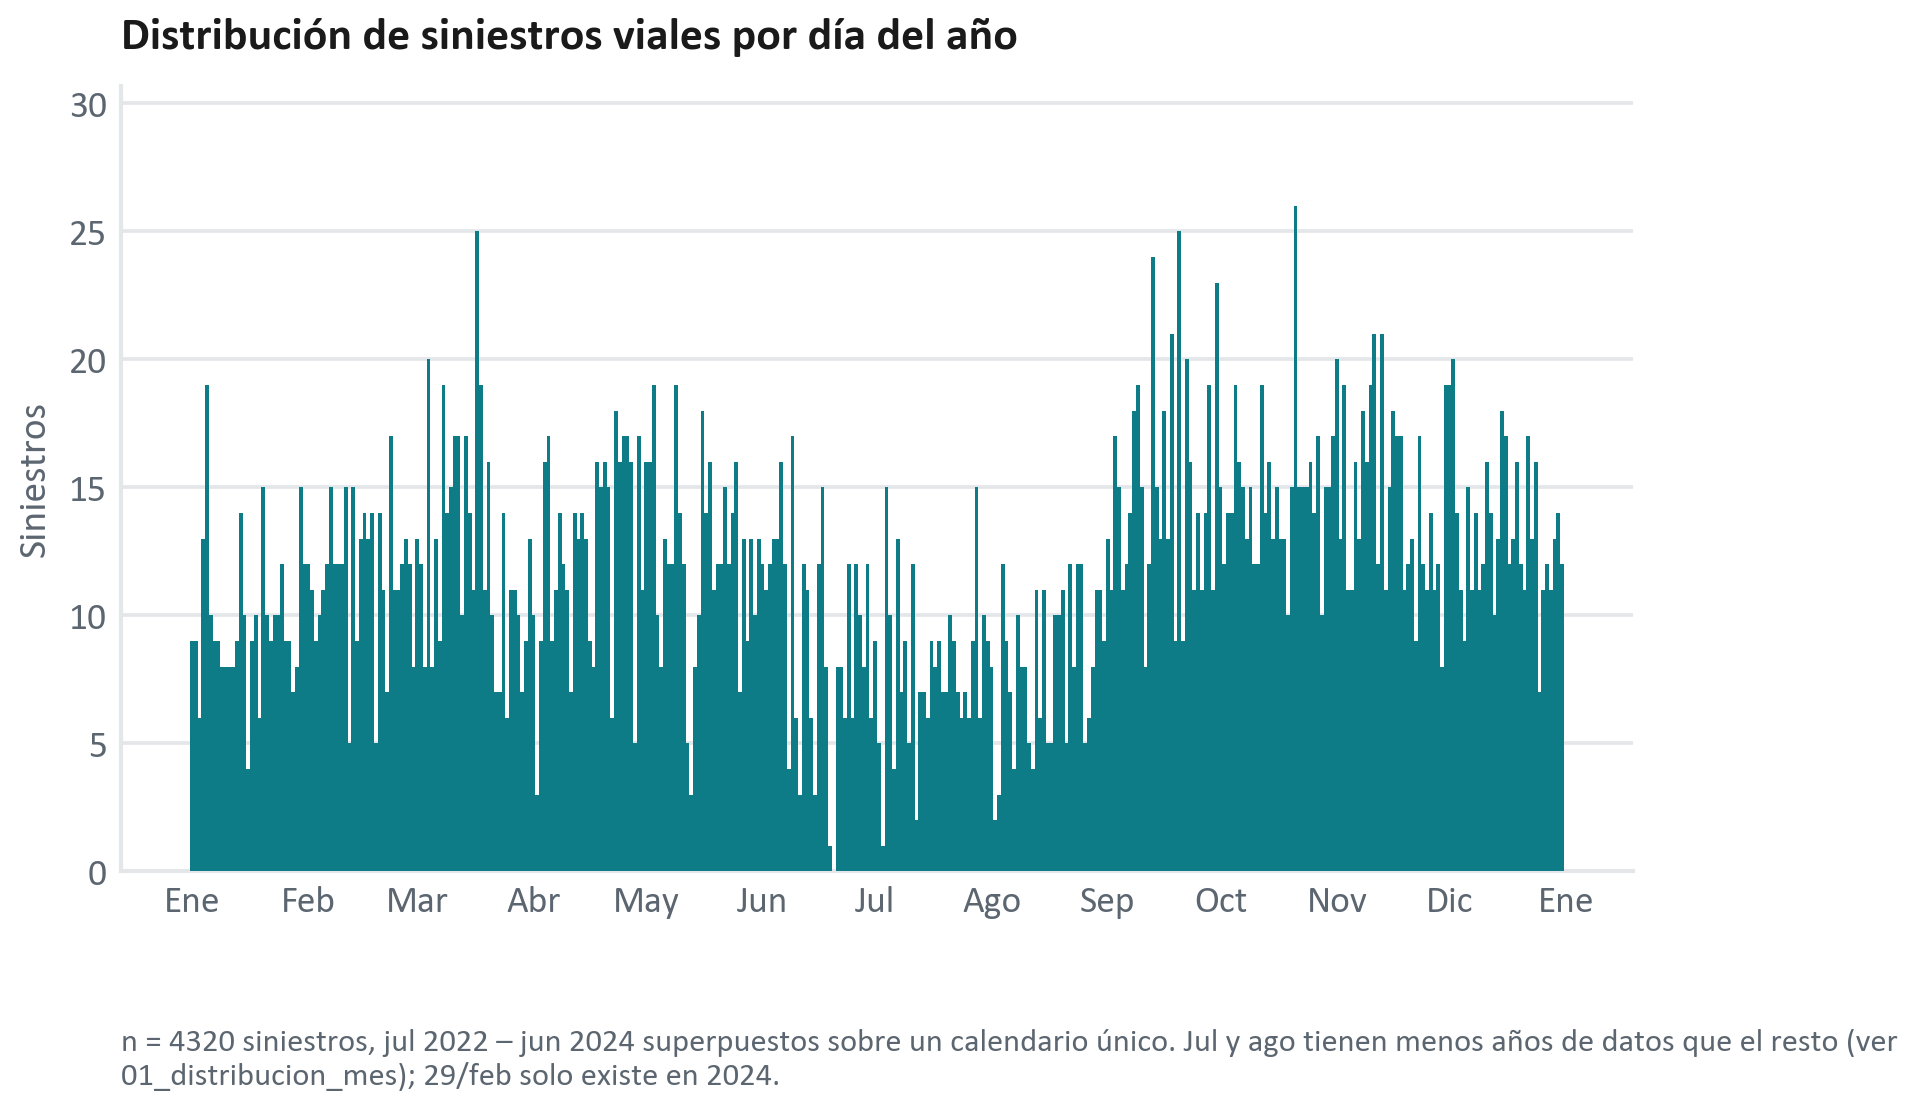
\includegraphics[width=0.85\linewidth]{imagenes/anexo_a2_distribucion_dia_anio.png}
\caption{Distribución de siniestros viales por día del año}
\label{fig:anexo-distribucion-dia-anio}
\notaflot{Frecuencia diaria de siniestros superpuesta sobre un calendario único de 365
días (n = 4320). Julio y agosto acumulan menos años de datos que el resto del
calendario, y el 29 de febrero solo existe en el año 2024, por lo que esos días deben
interpretarse con esa salvedad. Se observa mayor concentración entre septiembre y
noviembre. \fuentepropia{}.}
\end{figure}

\begin{figure}[htbp]
\centering
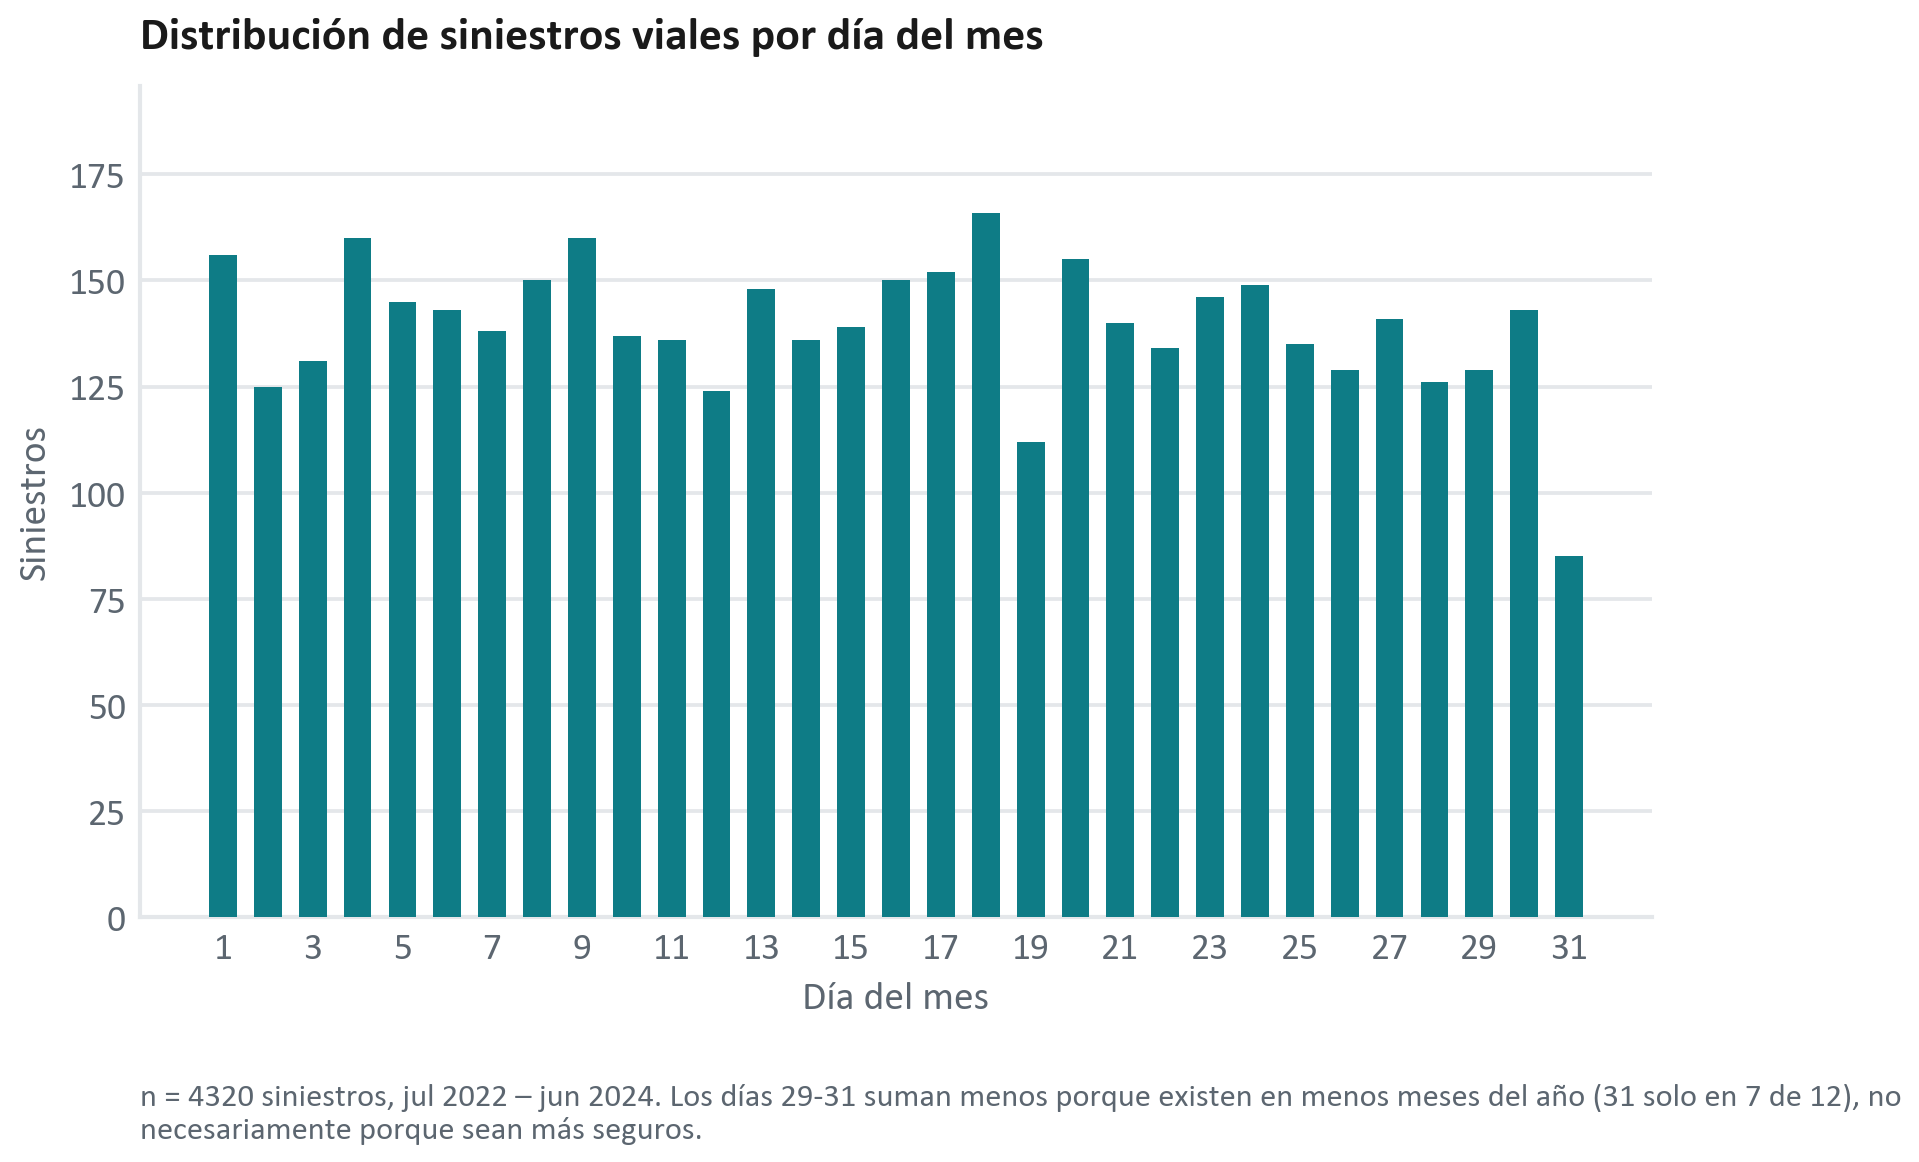
\includegraphics[width=0.85\linewidth]{imagenes/anexo_a2_distribucion_dia_mes.png}
\caption{Distribución de siniestros viales por día del mes}
\label{fig:anexo-distribucion-dia-mes}
\notaflot{Frecuencia de siniestros según el número de día calendario, sin distinguir
el mes (n = 4320). La distribución es relativamente uniforme entre los días 1 y 28; la
caída hacia el día 31 responde a que ese día solo existe en 7 de los 12 meses del año,
y no a un efecto real sobre la siniestralidad. \fuentepropia{}.}
\end{figure}

\begin{figure}[htbp]
\centering
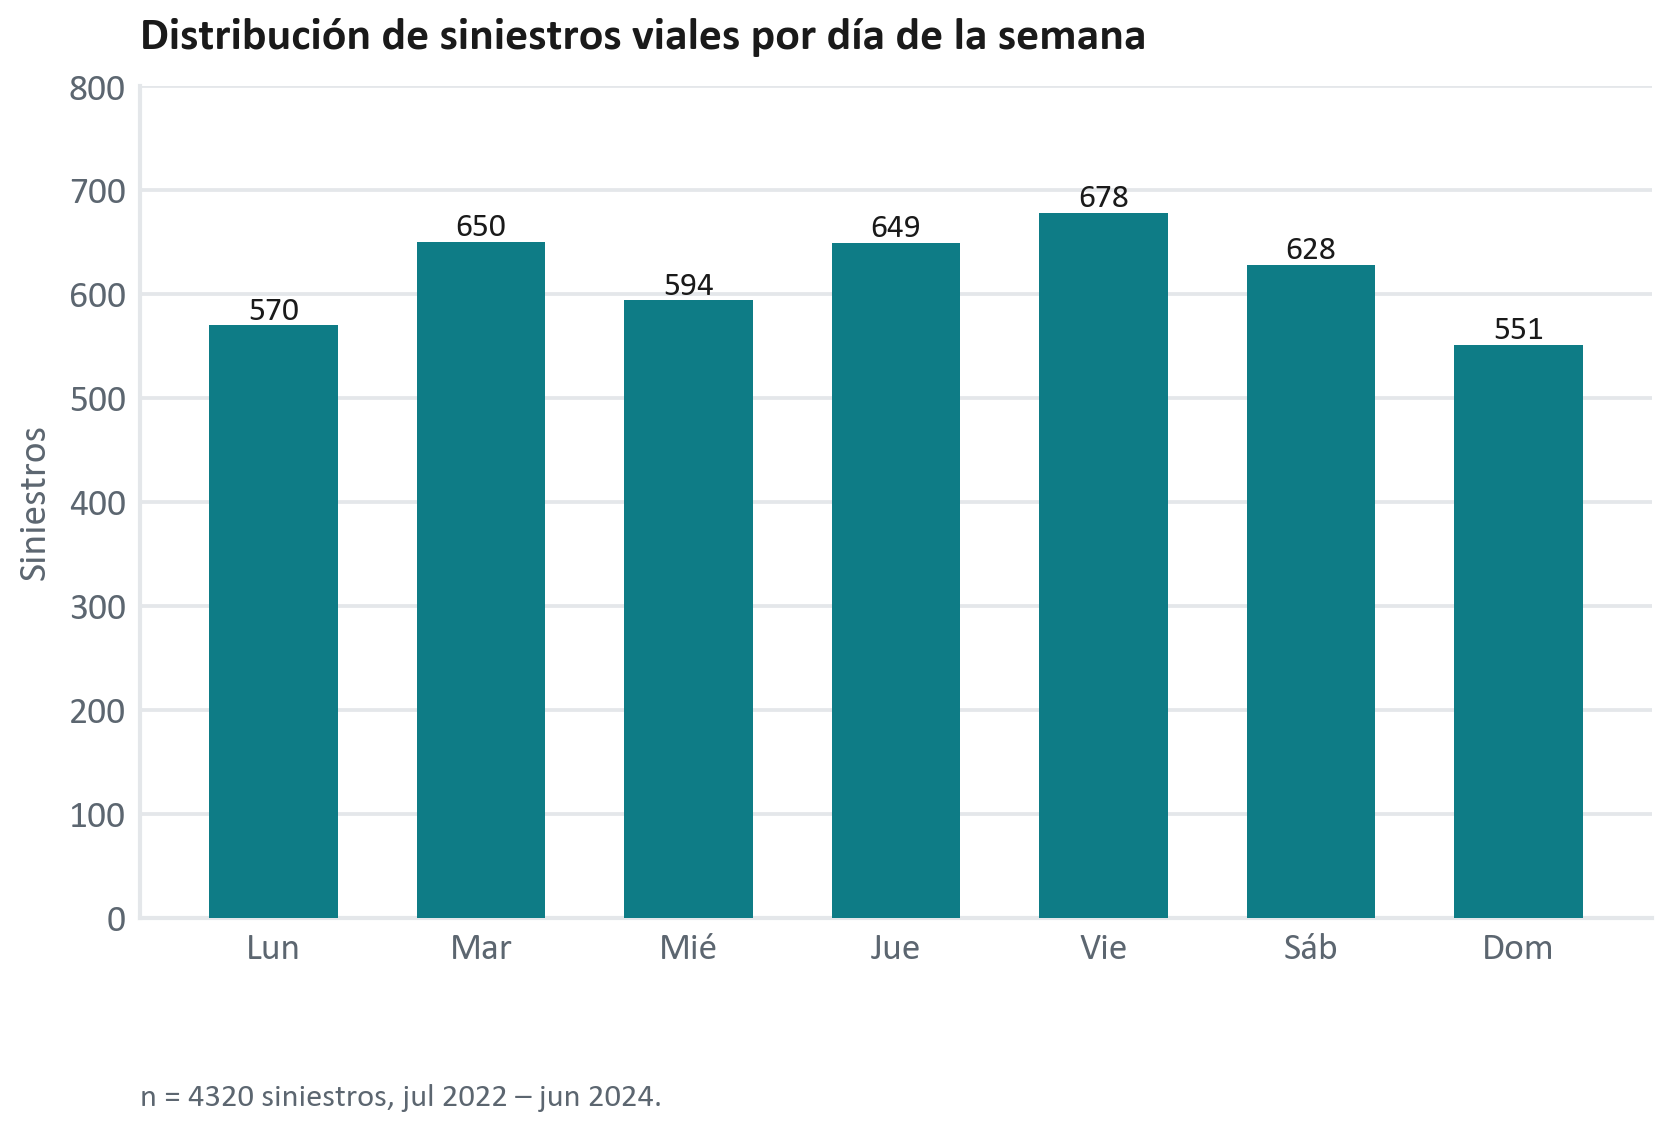
\includegraphics[width=0.85\linewidth]{imagenes/anexo_a2_distribucion_dia_semana.png}
\caption{Distribución de siniestros viales por día de la semana}
\label{fig:anexo-distribucion-dia-semana}
\notaflot{Frecuencia según día de la semana (n = 4320). El viernes concentra el máximo
(678) y el domingo el mínimo (551), con una distribución por lo demás relativamente
pareja entre martes y sábado. \fuentepropia{}.}
\end{figure}

\begin{figure}[htbp]
\centering
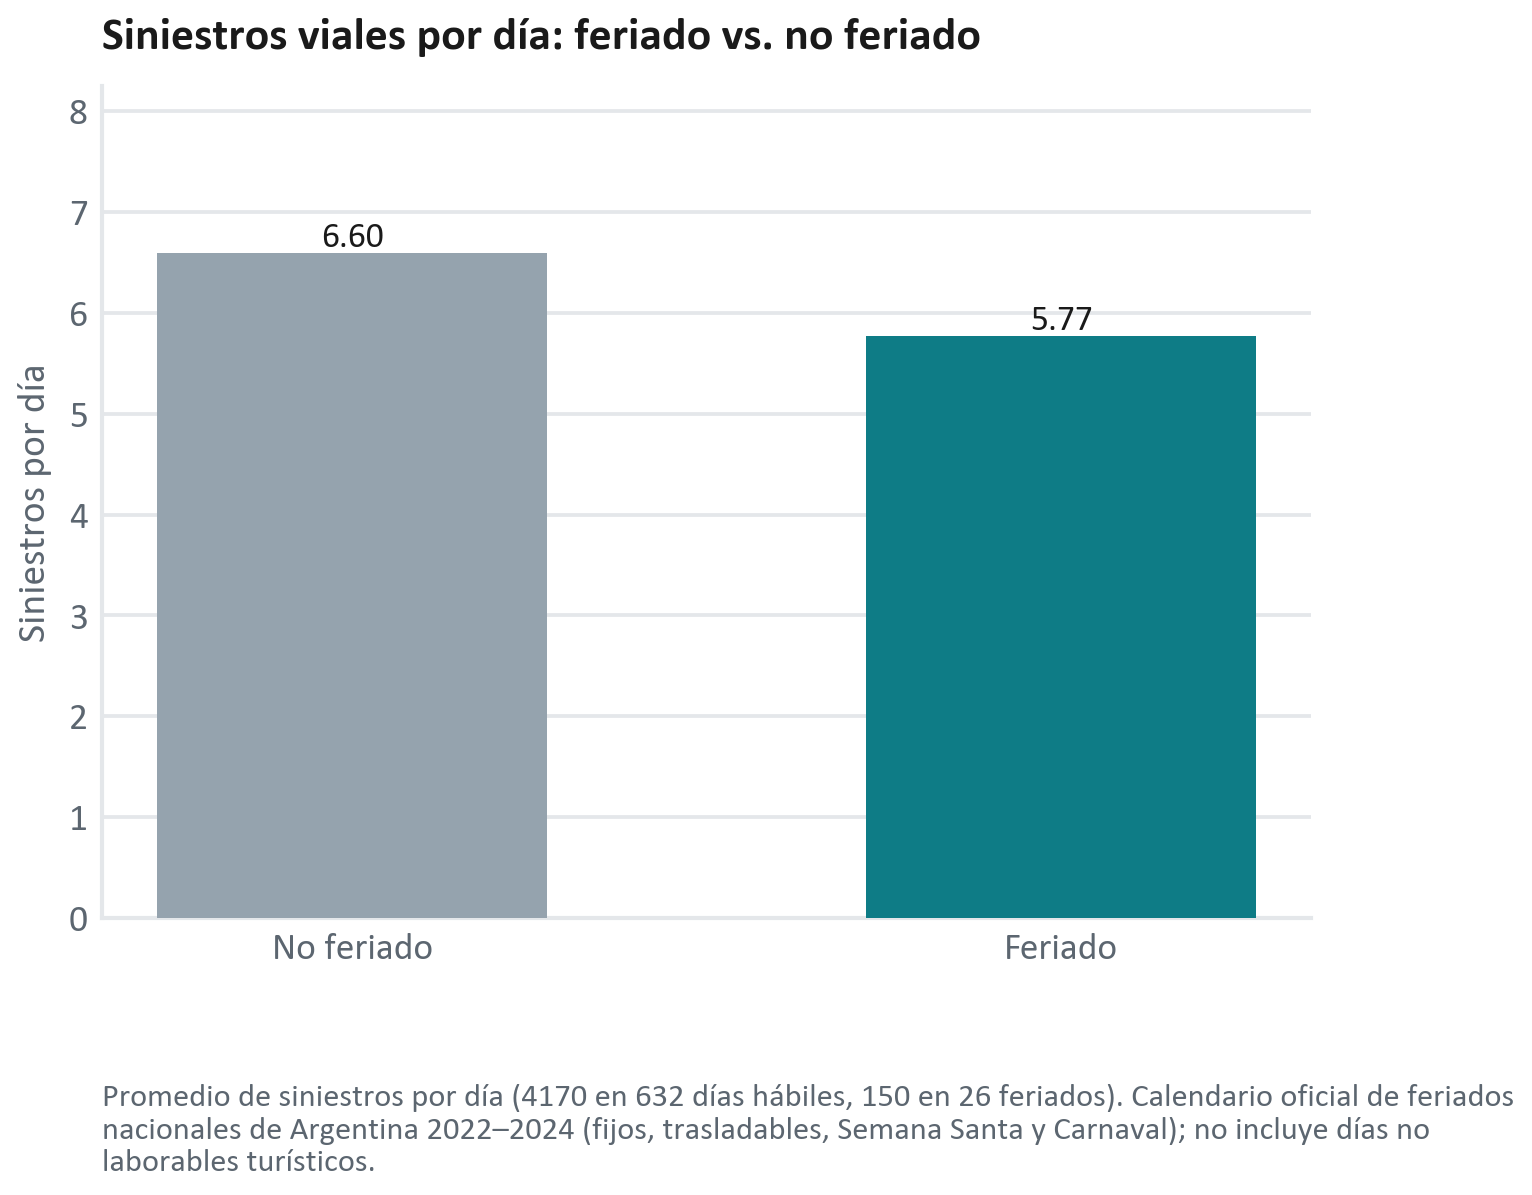
\includegraphics[width=0.75\linewidth]{imagenes/anexo_a2_feriado.png}
\caption{Siniestros viales por día: feriado frente a no feriado}
\label{fig:anexo-feriado}
\notaflot{Promedio de siniestros por día calendario, distinguiendo feriados
nacionales de días no feriados (4170 siniestros en 632 días hábiles y 150 en 26
feriados, según el calendario oficial de feriados de Argentina 2022--2024; no se
incluyen días no laborables turísticos). El promedio diario resulta levemente menor en
los feriados (5,77 frente a 6,60). \fuentepropia{}.}
\end{figure}

\begin{figure}[htbp]
\centering
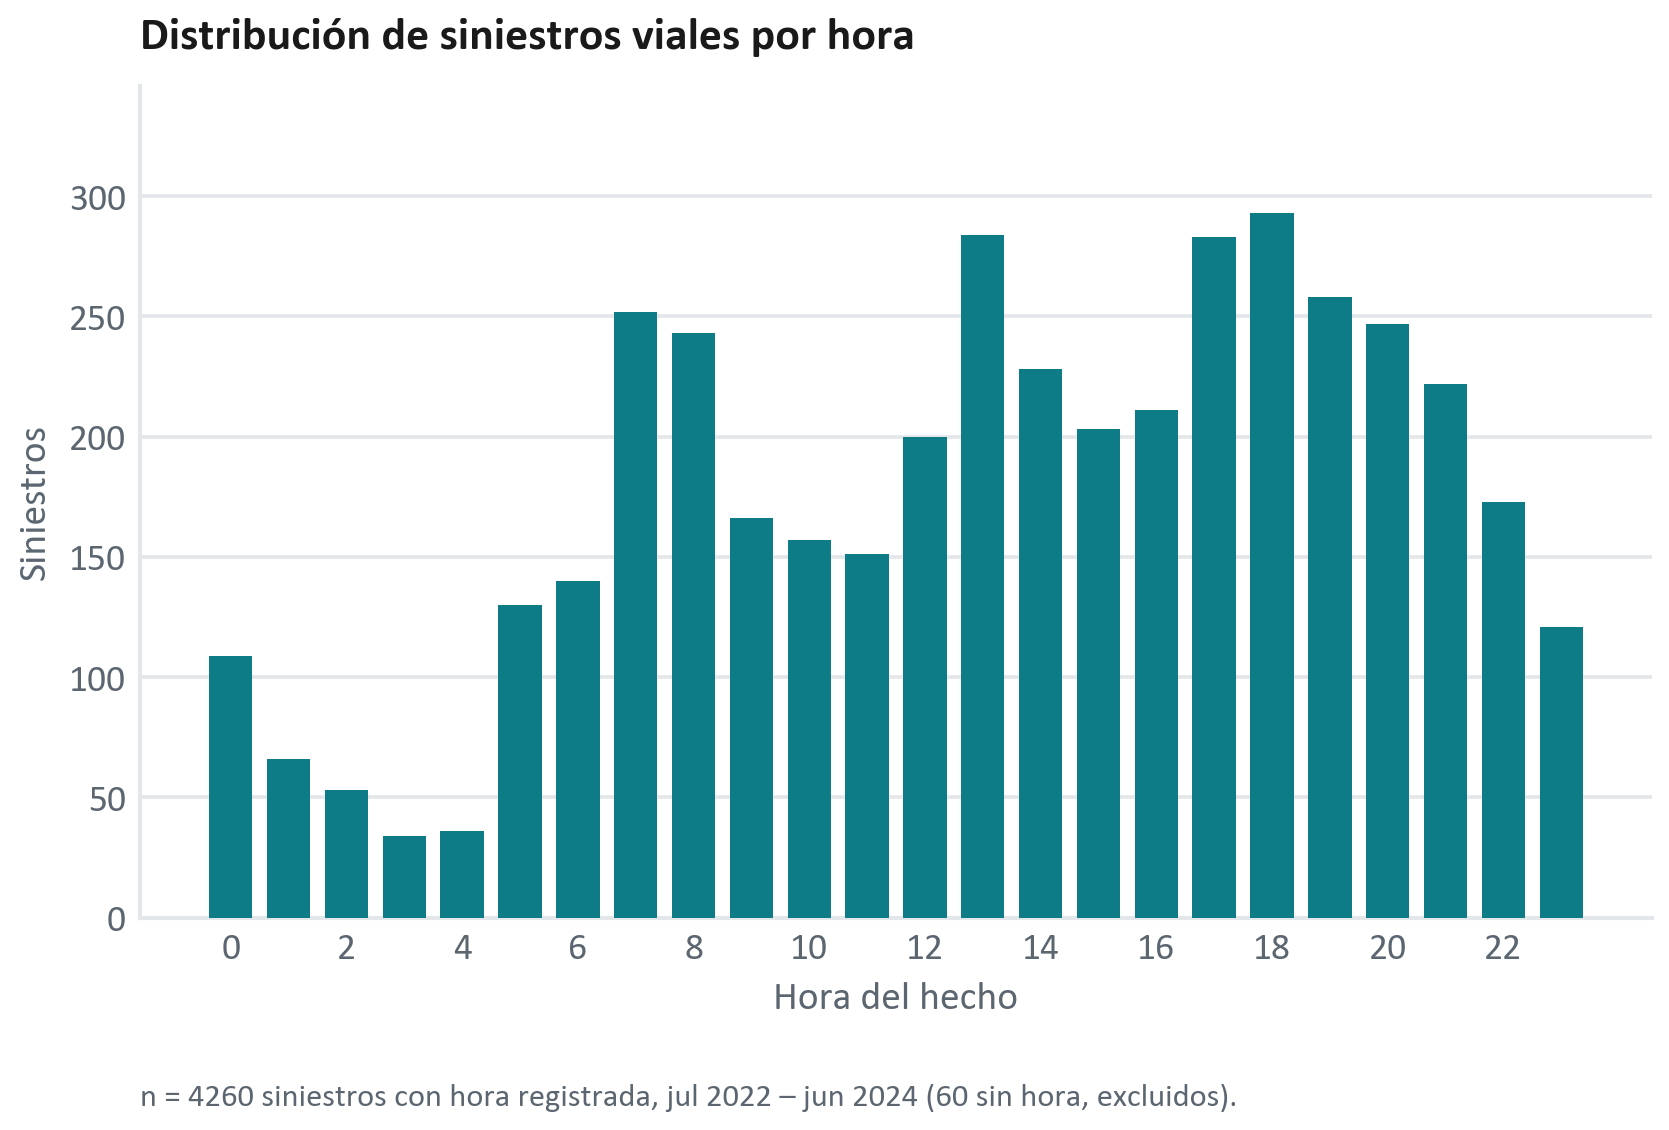
\includegraphics[width=0.85\linewidth]{imagenes/anexo_a2_distribucion_hora.png}
\caption{Distribución de siniestros viales por hora del hecho}
\label{fig:anexo-distribucion-hora}
\notaflot{Frecuencia horaria de los siniestros con hora registrada (n = 4260; 60 casos
sin dato, excluidos), julio 2022 -- junio 2024. Se identifican dos picos, uno hacia el
mediodía (13 h) y otro más pronunciado al final de la tarde (18 h), coincidentes con
los horarios de mayor circulación, y un mínimo en la madrugada (3--4 h). \fuentepropia{}.}
\end{figure}

\begin{figure}[htbp]
\centering
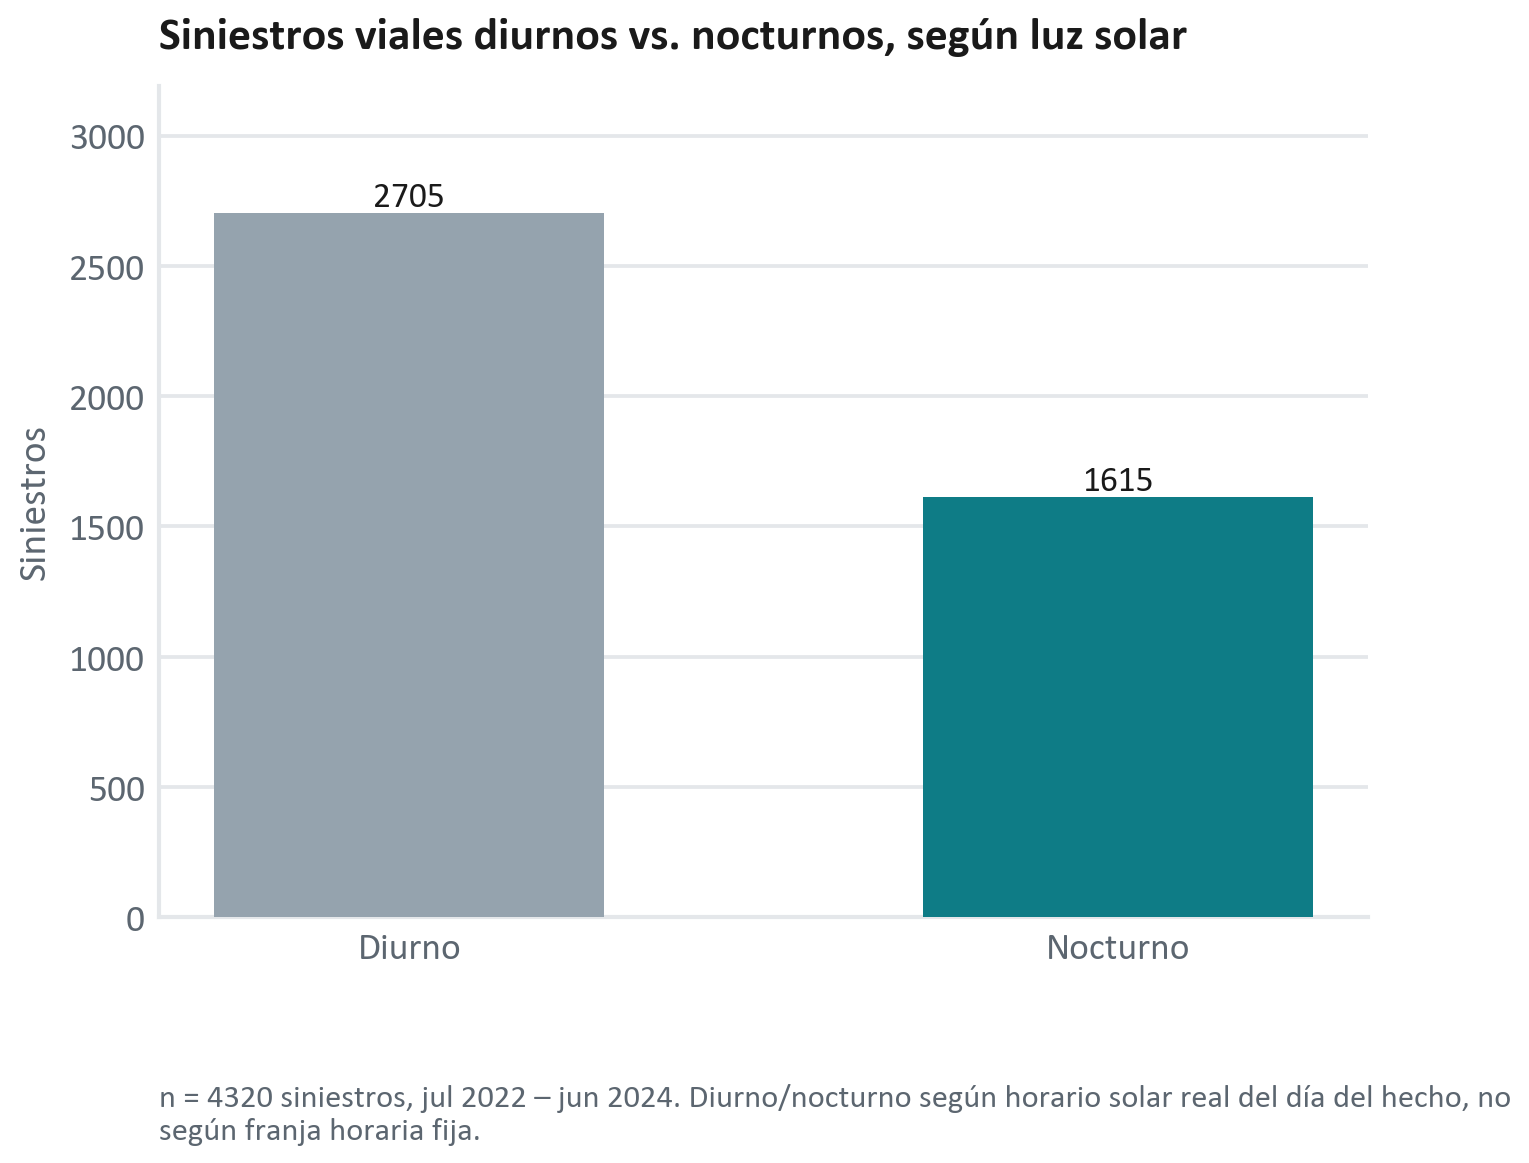
\includegraphics[width=0.7\linewidth]{imagenes/anexo_a2_diurno_nocturno.png}
\caption{Siniestros viales diurnos frente a nocturnos, según luz solar}
\label{fig:anexo-diurno-nocturno}
\notaflot{Clasificación de los 4320 siniestros según el horario solar real del día en
que ocurrieron, y no según una franja horaria fija. Un 63\,\% de los casos (2705)
ocurre en horario diurno y el 37\,\% restante (1615) en horario nocturno. \fuentepropia{}.}
\end{figure}

\begin{figure}[htbp]
\centering
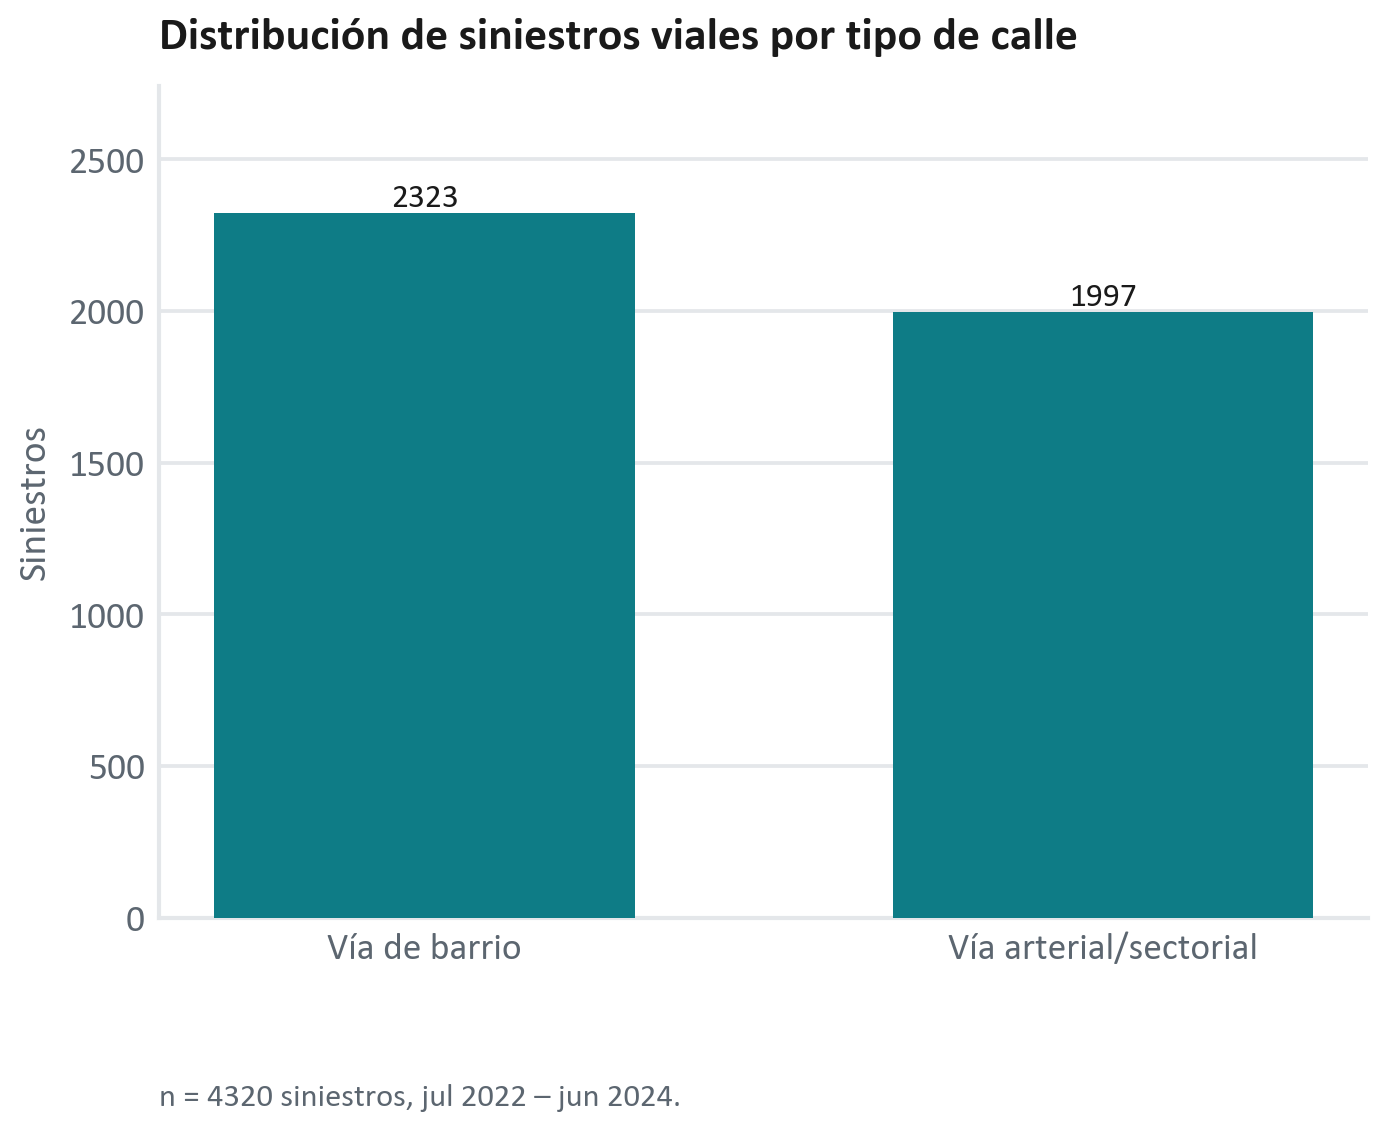
\includegraphics[width=0.78\linewidth]{imagenes/anexo_a2_tipo_calle.png}
\caption{Distribución de siniestros viales por tipo de calle}
\label{fig:anexo-tipo-calle}
\notaflot{Clasificación según jerarquía vial (n = 4320). Las vías de barrio concentran
algo más de la mitad de los casos (2323) frente a las vías arteriales o sectoriales
(1997), lo que confirma que el fenómeno no se limita a los corredores principales.
\fuentepropia{}.}
\end{figure}

\begin{figure}[htbp]
\centering
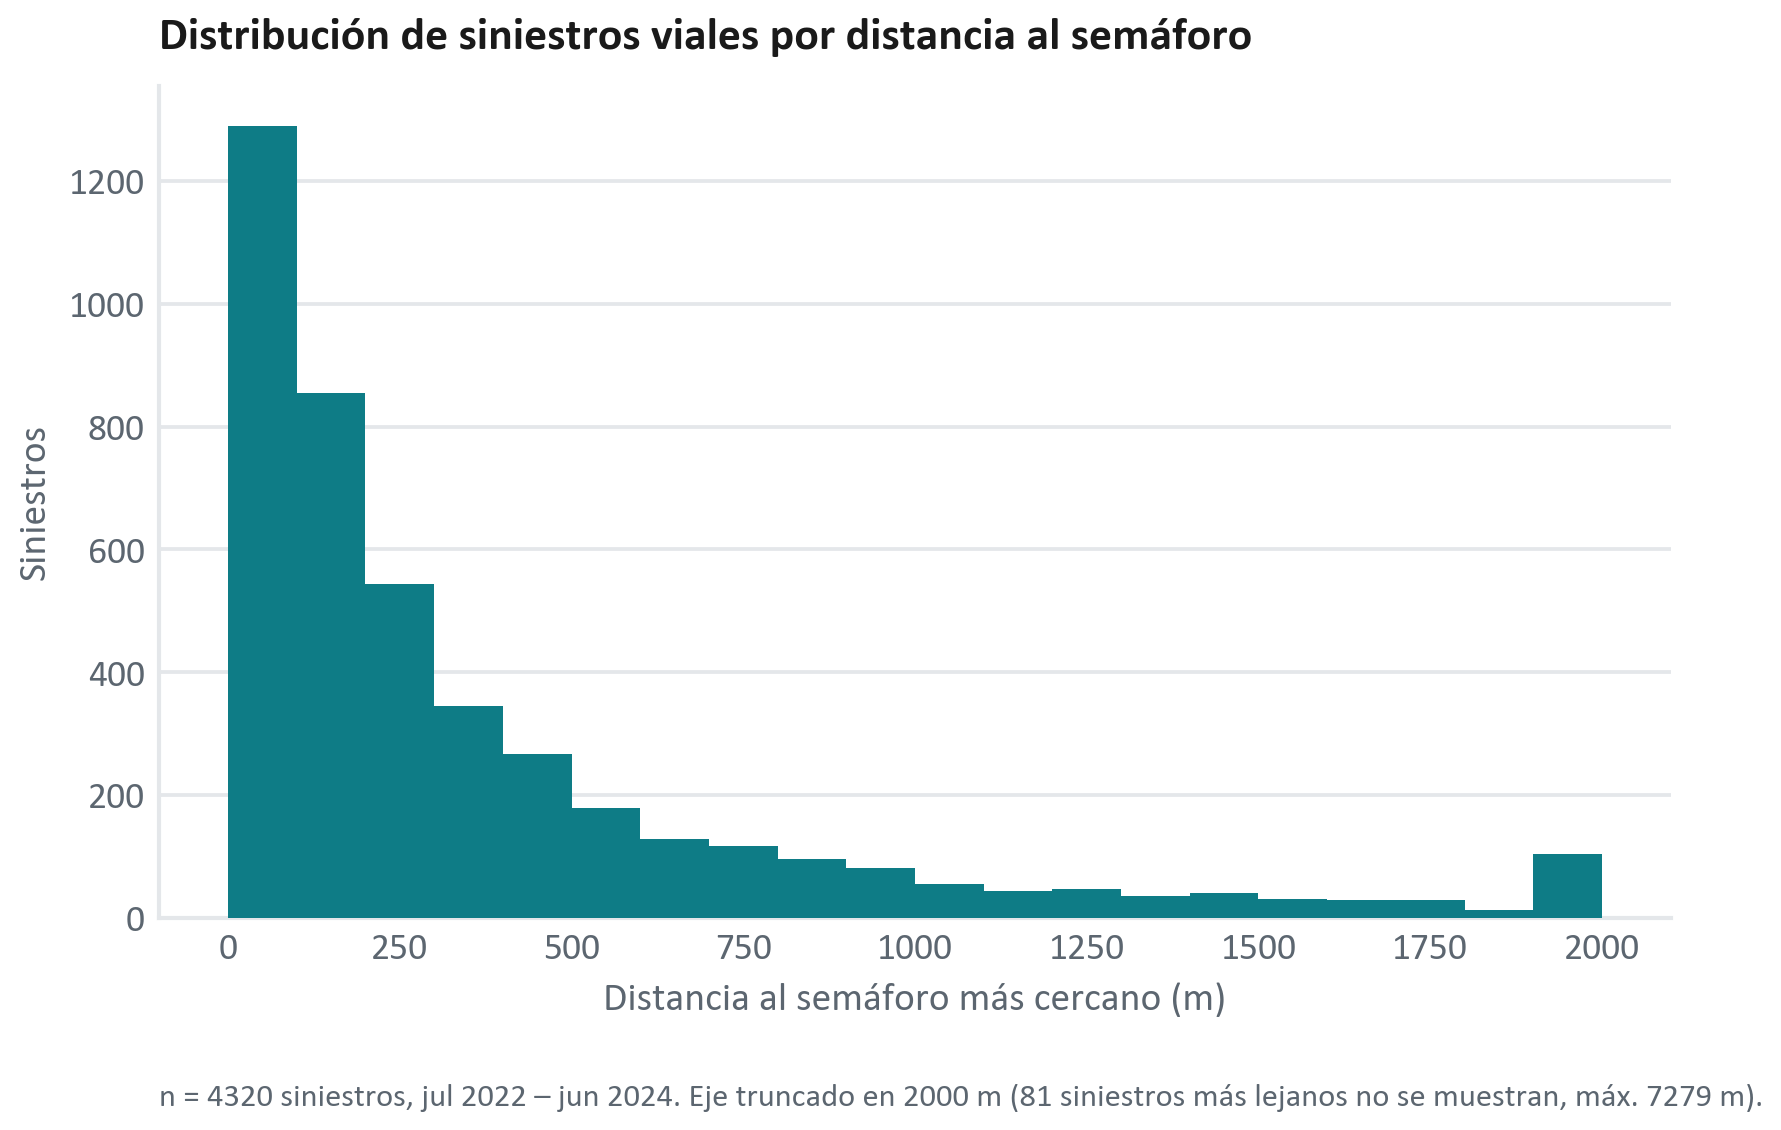
\includegraphics[width=0.8\linewidth]{imagenes/anexo_a2_distancia_semaforo.png}
\caption{Distribución de siniestros viales por distancia al semáforo más cercano}
\label{fig:anexo-distancia-semaforo}
\notaflot{Histograma de la distancia radial de cada siniestro al semáforo más cercano
(n = 4320; eje truncado en 2000 m, lo que deja fuera 81 casos más lejanos, con un
máximo de 7279 m). La frecuencia decrece marcadamente con la distancia: casi un
tercio de los siniestros ocurre a menos de 100 m de un semáforo. \fuentepropia{}.}
\end{figure}

\begin{figure}[htbp]
\centering
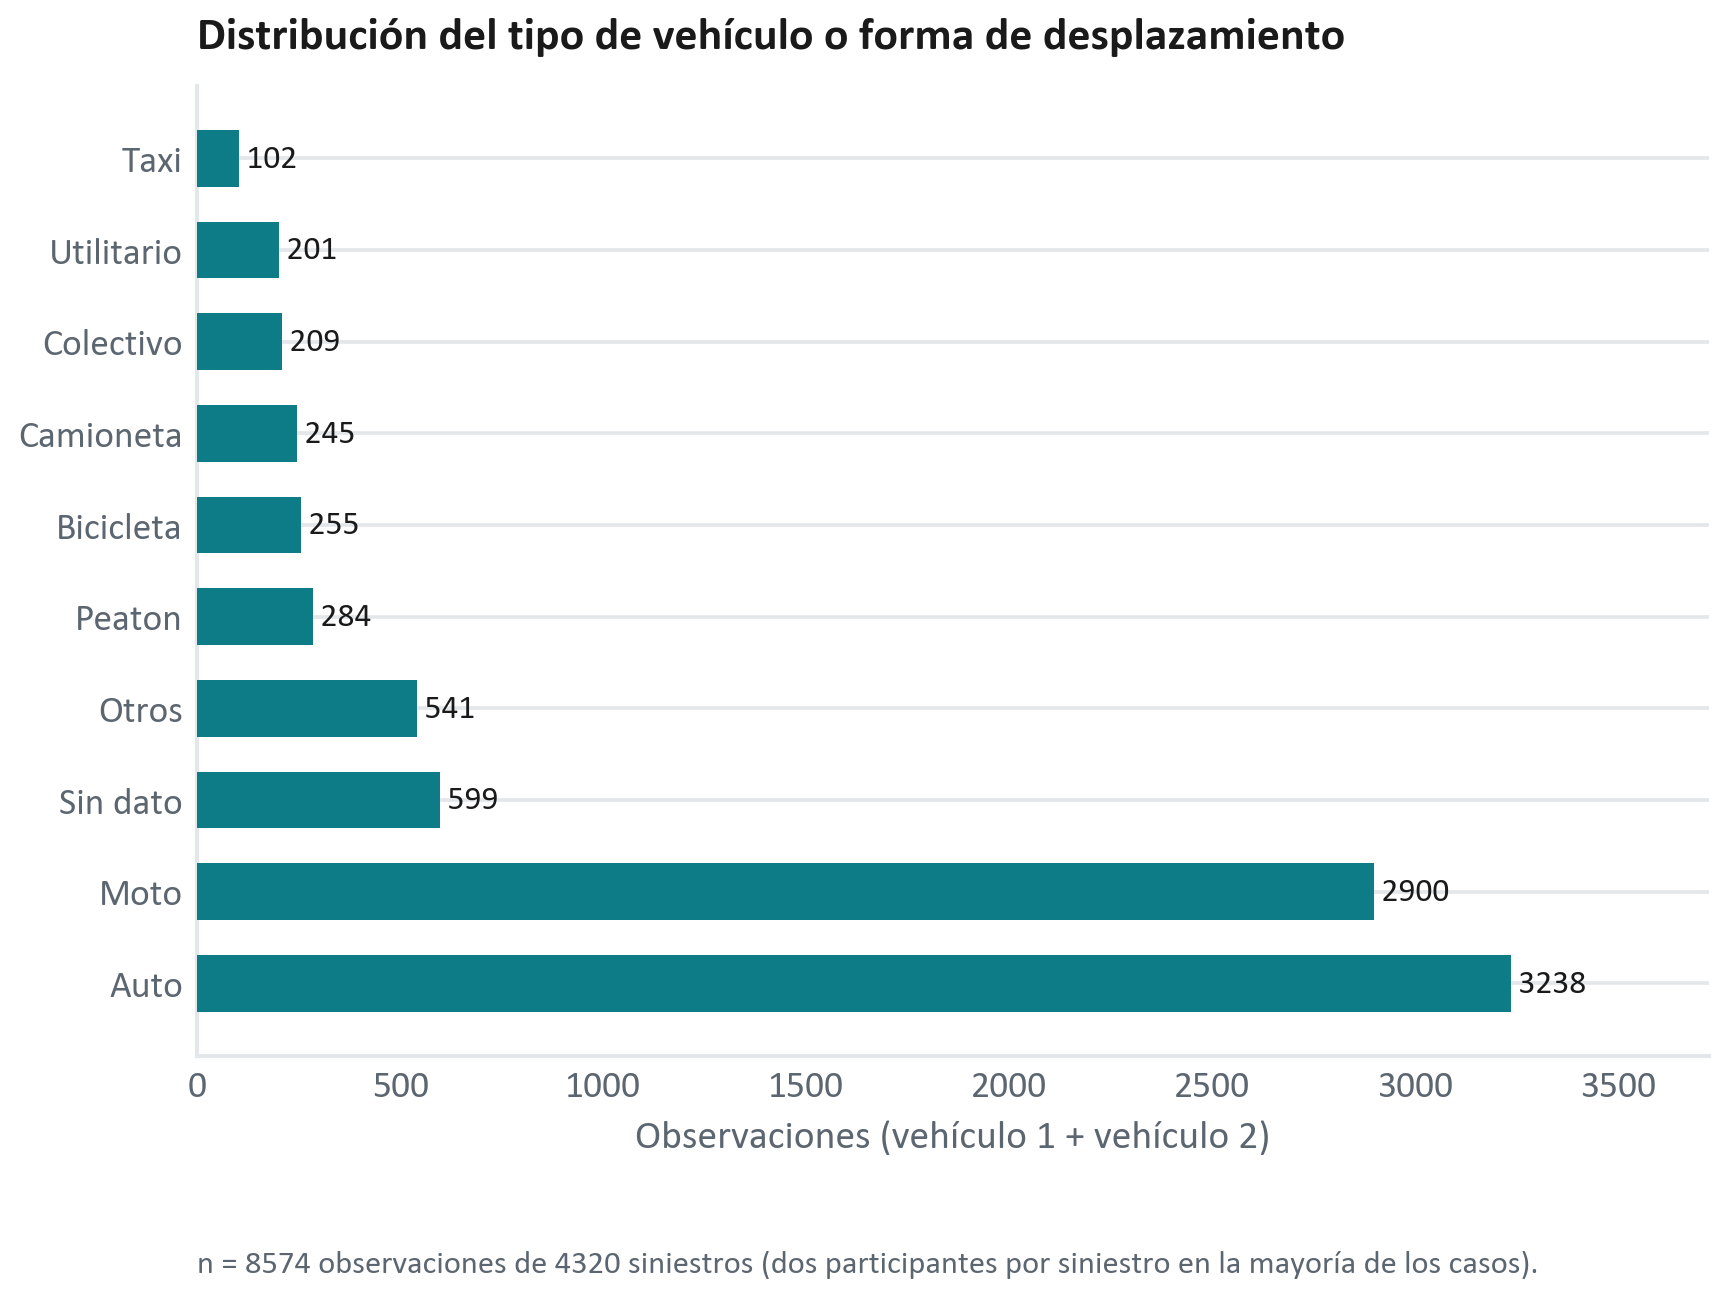
\includegraphics[width=0.8\linewidth]{imagenes/anexo_a2_tipo_vehiculo.png}
\caption{Distribución del tipo de vehículo o forma de desplazamiento}
\label{fig:anexo-tipo-vehiculo}
\notaflot{Participaciones registradas en los 4320 siniestros (n = 8574 observaciones,
correspondientes a vehículo 1 y vehículo 2 cuando corresponde). La unidad de conteo es
la participación y no el siniestro, por lo que las categorías no son excluyentes entre
sí. Los automóviles (3238) y las motocicletas (2900) concentran la mayor parte de las
observaciones. \fuentepropia{}.}
\end{figure}

\begin{figure}[htbp]
\centering
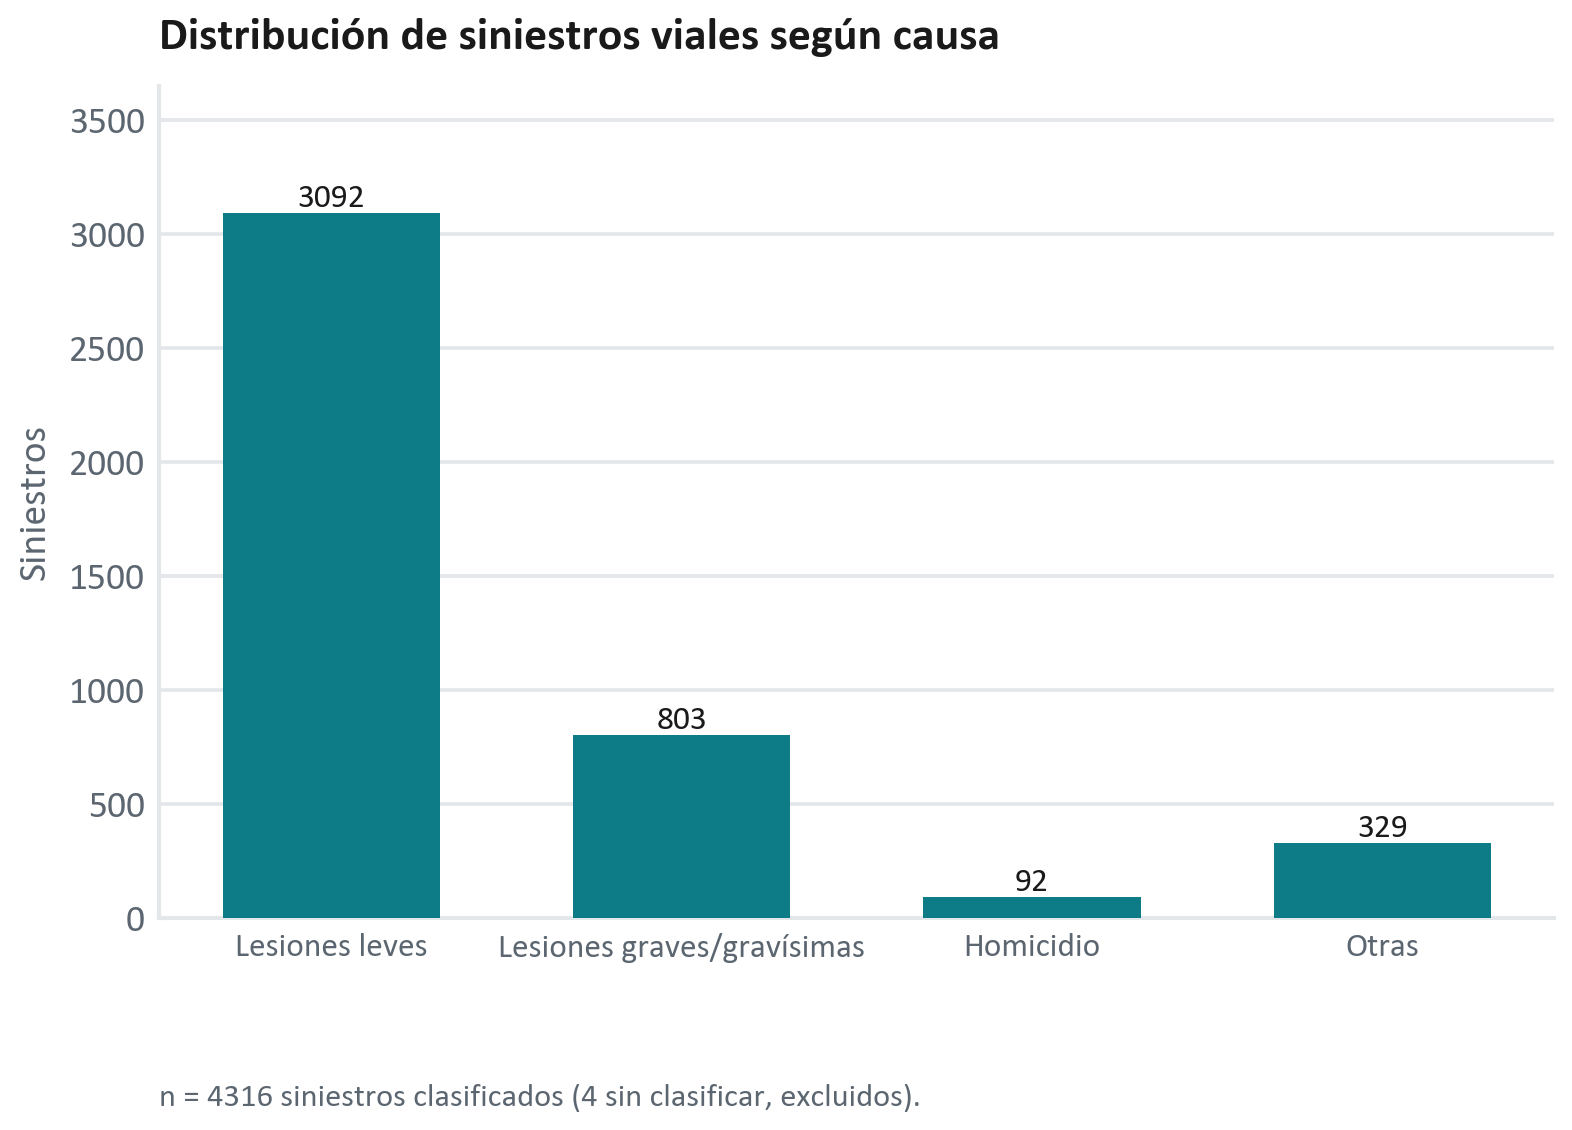
\includegraphics[width=0.75\linewidth]{imagenes/anexo_a2_causa.png}
\caption{Distribución de siniestros viales según causa}
\label{fig:anexo-causa}
\notaflot{Clasificación según la carátula asignada en la causa judicial (n = 4316; 4
casos sin clasificar, excluidos). Predominan las lesiones leves (3092), seguidas por
las lesiones graves o gravísimas (803), otras carátulas (329) y el homicidio culposo
(92). \fuentepropia{}.}
\end{figure}

\begin{figure}[htbp]
\centering
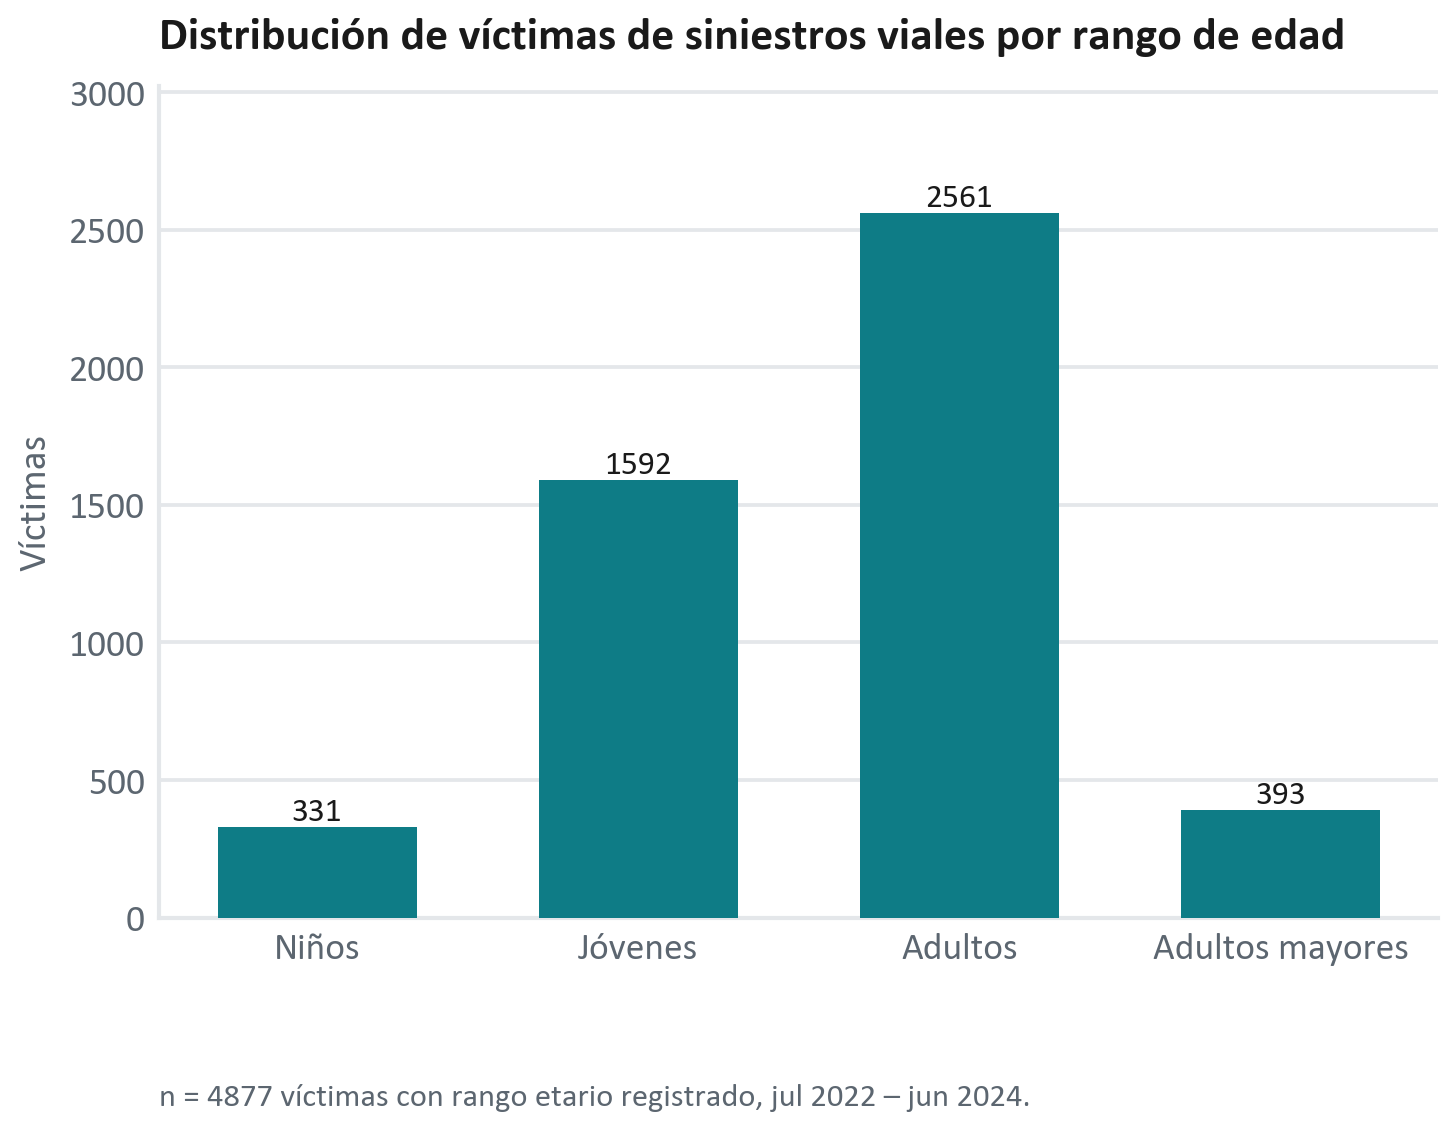
\includegraphics[width=0.75\linewidth]{imagenes/anexo_a2_rango_edad.png}
\caption{Distribución de víctimas de siniestros viales por rango etario}
\label{fig:anexo-rango-edad}
\notaflot{Distribución etaria de las víctimas con dato de edad registrado (n = 4877),
según los rangos definidos por la Organización Mundial de la Salud. Los adultos (27 a
59 años) concentran la mayor cantidad de víctimas (2561), seguidos por los jóvenes de
15 a 26 años (1592). \fuentepropia{}.}
\end{figure}

\begin{figure}[htbp]
\centering
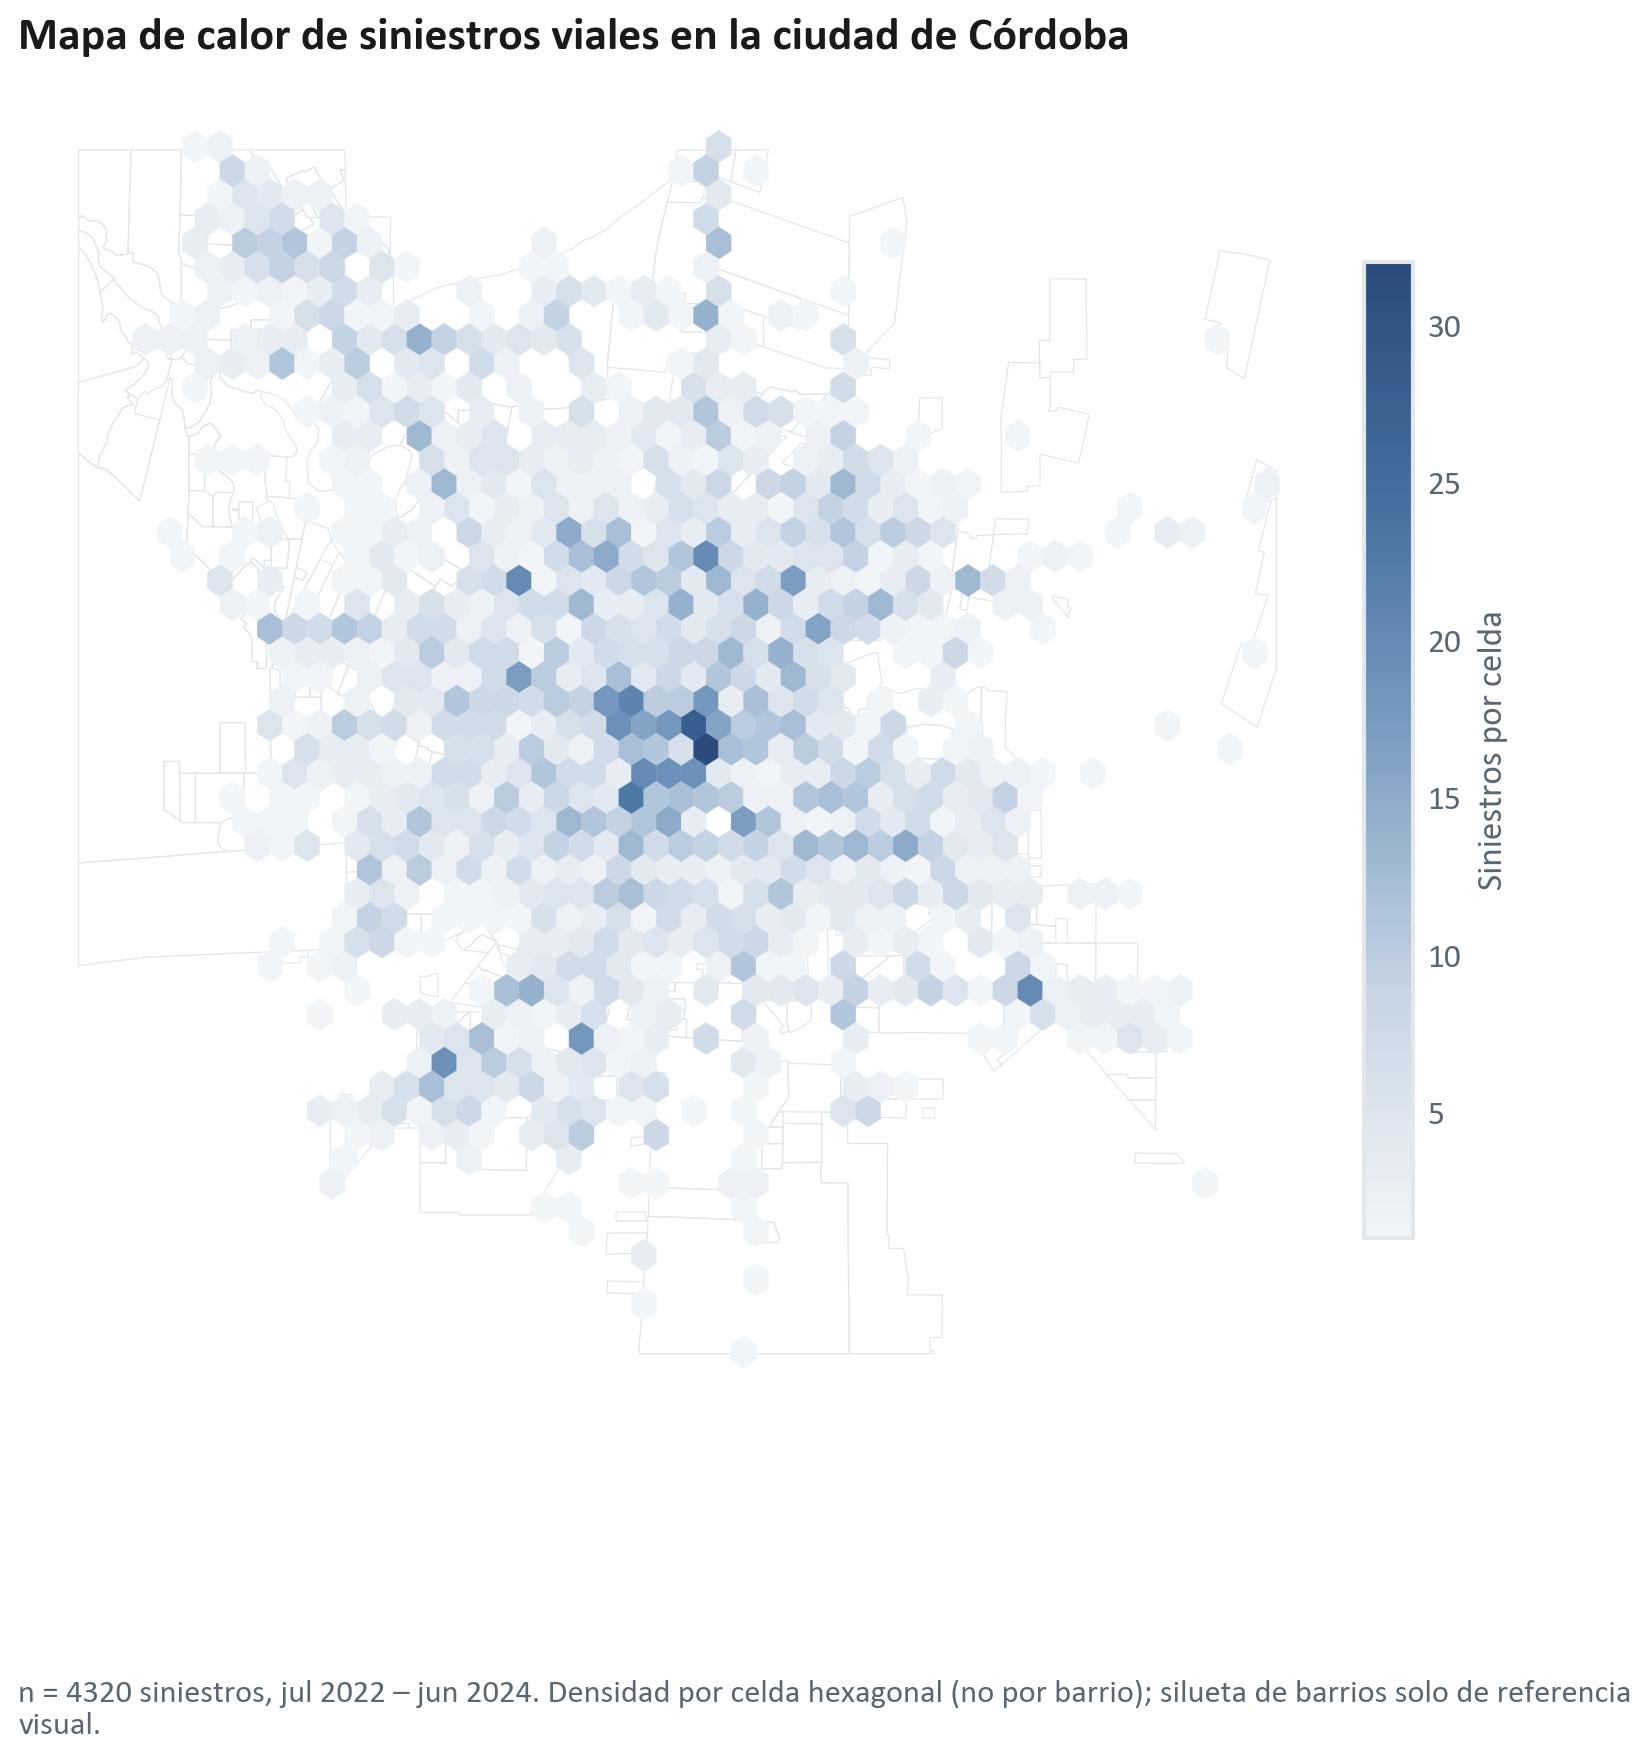
\includegraphics[width=0.62\linewidth]{imagenes/anexo_a2_mapa_calor_ciudad.png}
\caption{Mapa de calor de siniestros viales en la ciudad de Córdoba}
\label{fig:anexo-mapa-calor-ciudad}
\notaflot{Densidad espacial de los 4320 siniestros georreferenciados, agregada por
celda hexagonal de superficie constante; la silueta de barrios se incluye solo como
referencia visual. Se observa una concentración marcada en el área central, con
máximos puntuales superiores a 30 siniestros por celda. \fuentepropia{}.}
\end{figure}

\begin{figure}[htbp]
\centering
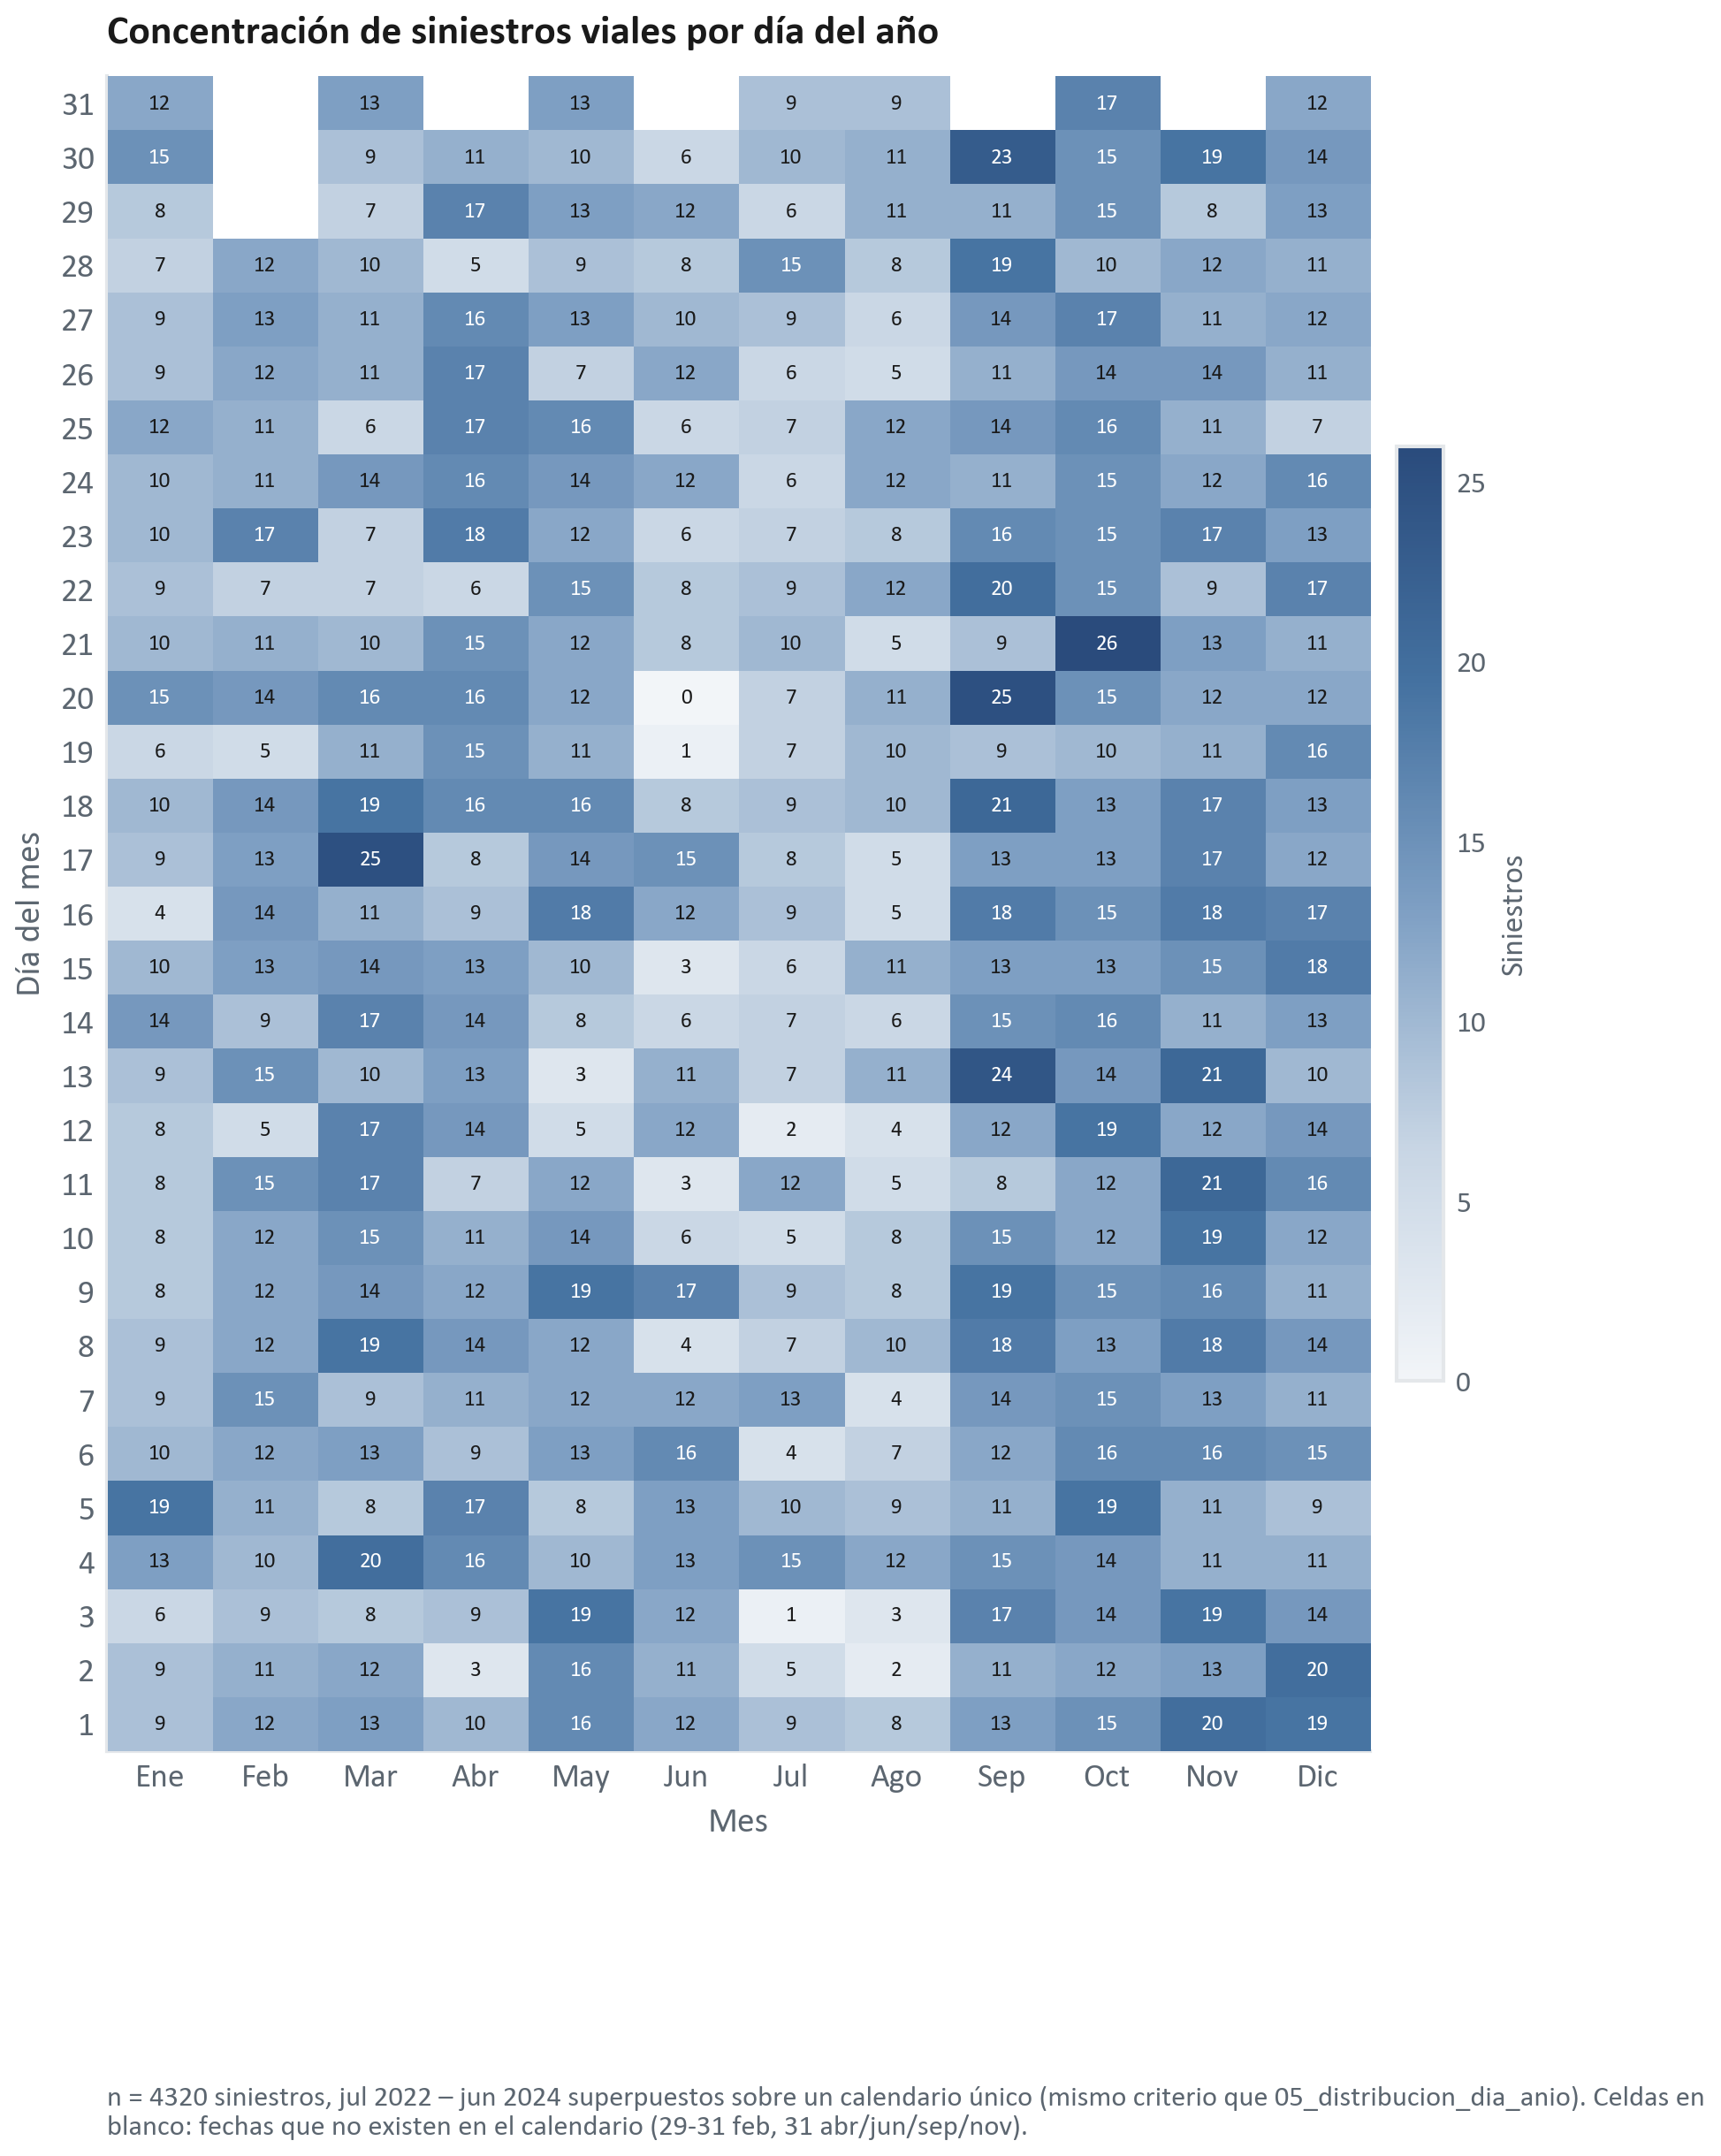
\includegraphics[width=0.7\linewidth]{imagenes/anexo_a2_mapa_calor_dia_anio.png}
\caption{Concentración de siniestros viales por día del año}
\label{fig:anexo-mapa-calor-dia-anio}
\notaflot{Representación matricial (mes por día del mes) de la misma distribución
diaria presentada en la \cref{fig:anexo-distribucion-dia-anio} (n = 4320, mismo
criterio de superposición sobre un calendario único). Las celdas en blanco
corresponden a fechas que no existen en el calendario (29 a 31 de febrero, y el día 31
de abril, junio, septiembre y noviembre). \fuentepropia{}.}
\end{figure}
